\documentclass[a4paper, 10pt, fleqn]{article}

\usepackage[utf8]{inputenc}
\usepackage[T1]{fontenc}
\usepackage{textcomp}
\usepackage{lmodern}
\usepackage[ngerman]{babel}
\usepackage{enumerate}
\usepackage{xcolor}

\usepackage{amsmath}
\usepackage{graphicx}
\usepackage{subcaption}
\usepackage{geometry}
\usepackage{scrpage2}
\usepackage{lastpage}
\usepackage[hyphens]{url}
\usepackage{hyperref}
\usepackage{listings}
\lstset{language=[ansi]C++}

\geometry{left=3cm, top=3cm, bottom=3cm, right=2cm}

\hypersetup{
    colorlinks,
    linkcolor=black,
    citecolor=black,
    urlcolor=black
}


\pagestyle{scrheadings}
\ihead{PREN1 Gruppe 39}\ohead{Technologierecherche} 
\ifoot{3. Januar 2016} \ofoot{Seite \thepage\ von \pageref{LastPage}}


\begin{document}
\input{titlepageTR.tex}
\tableofcontents
\clearpage
%% !TEX root = Technologierecherche.tex
\section*{Abstract}
%% !TEX root = Technologierecherche.tex
\section{Einleitung}
% !TEX root = Technologierecherche.tex
\section{Autonomes Fahren}
% !TEX root = Technologierecherche.tex
\section{Spurerkennung}
% !TEX root = Technologierecherche.tex
\subsection{Rechtsvortritt}

% !TEX root = Technologierecherche.tex
\section{Beladen}
\subsection{Erkennung des Containers}
\textbf {Mit Distanzsensoren und Farbsensoren}
\begin{itemize}
\item Unbekannte Genauigkeit muss getestet werden.
\item Benötigt AD Wandler (Wenn Infrarot- oder Ultraschallsensor)
\item Kein mechanischer Kontakt
\end{itemize}
\begin{figure}[h]
	\centering
	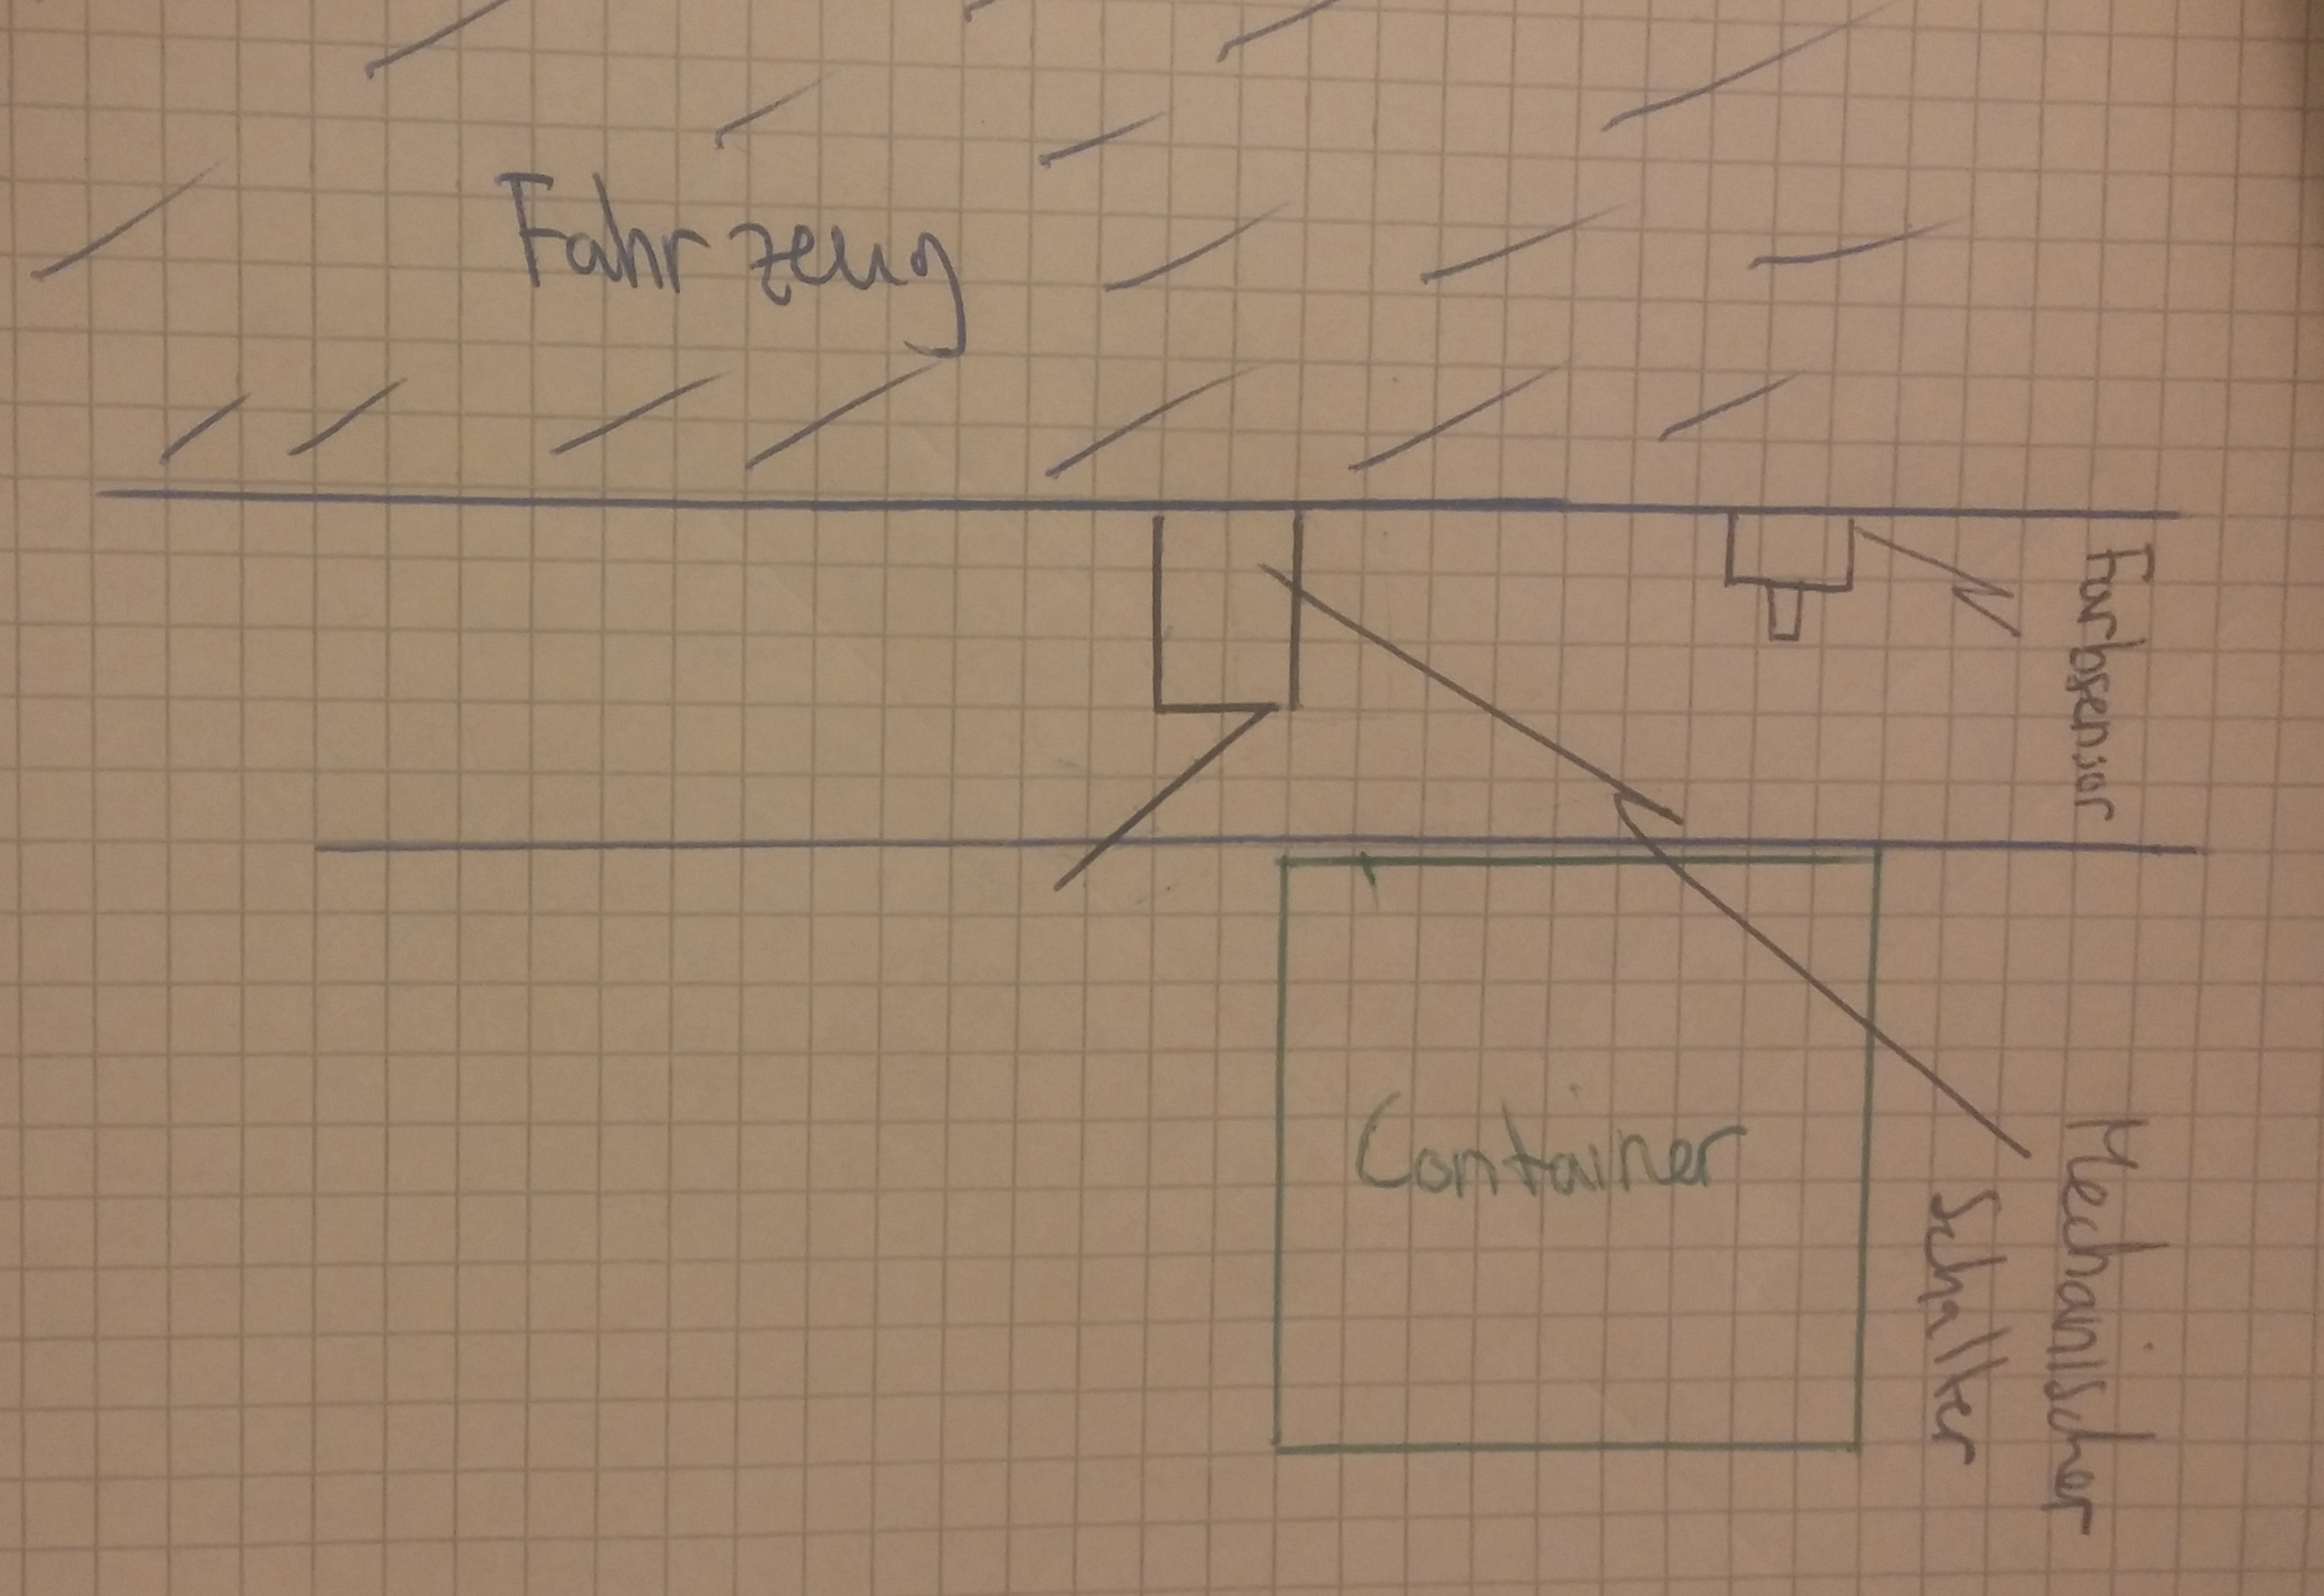
\includegraphics[width=0.5\textwidth]{Images/Containererkennung_1.png}
	\caption{Distanzsensoren an der rechten Seite des Fahrzeugs}
\end{figure}

\textbf {Mechanische Detektion und Farbsensoren}
\begin{itemize}
\item Unbekannte Genauigkeit muss getestet werden.
\item Klarer Wert
\item Mechanischer Kontakt (darf nichts ausser den Container berühren)
\end{itemize}
\begin{figure}[h]
	\centering
	\includegraphics[width=0.5\textwidth]{Images/Containererkennung_2.png}
	\caption{Ein Schalter an der rechten Seite des Fahrzeugs}
\end{figure}

\subsection{Mechanismen die bei Müllfahrzeugen eingesetzt werden}

\begin{itemize}
\item Der Greifer kann senkrecht zur Fahrbahn ausgefahren werden. Zudem ist der Greifer fähig eine Rotation um ca. 135° durchführen. 

Der genaue Mechanismus ist auf youtube (https://www.youtube.com/watch?v=LTUjiLxzDQs)  von 0.08 bis 0.23 ersichtlich.

\item Auf dem selben Video (bei 4:33-4:57) ist ein weiterer Mechanismus zu sehen, der mit einem Knickarm funktioniert. 

\item Bei 5:20-5:50 ist ein sehr einfache und direkte Lösung zu sehen. Es dürfte schwierig sein, diesen Vorgang autonom zu realisieren. 
\end{itemize}
% !TEX root = Technologierecherche.tex
\section{Entladen}
\subsection{Kippen des Behälters}

\includegraphics[width=0.5\textwidth]{Images/Entladen1.jpg}

Seitliches Entladen des Behälters

Vorteile:
\begin{itemize}
\item einfache Realisierung
\item wird in der Praxis angewandt
\end{itemize}

Nachteile:
\begin{itemize}
\item Nahes Heranfahren an Entladebehälter notwendig
\end{itemize}

\subsection{Seitliche Klappe öffnen}

Vorteil:
\begin{itemize}
\item sehr einfach realisierbar
\end{itemize}

\begin{flushleft}
Nachteile:
\end{flushleft}
\begin{itemize}
\item nicht automatisch wieder verschliessbar
\item fraglich ob Zielbereich einhaltbar ist
\end{itemize}

\subsection{Mit Greifer ausladen}

Vorteil:
\begin{itemize}
\item Greifer wird für 2 Funktion gebraucht (Einladen/Ausladen)
\end{itemize}

\begin{flushleft}
Nachteile:
\end{flushleft}
\begin{itemize}
\item schwierig gesamtes Schüttgut zu erwischen
\item aufwändiger Greifer
\item schwierig realisierbar
\end{itemize}
% !TEX root = Technologierecherche.tex
\section{Greifer}
\subsection{mechanisch}
Greifer besteht aus einer festen Seite und einer beweglichen Seite

\includegraphics[width=0.5\textwidth]{Images/Gripper6.png}

Eigenschaften: 
\begin{itemize}
\item sehr einfacher Aufbau
\item wenige Teile notwendig
\item nicht präzise Lösung
\end{itemize}

Greifer mittels 2 Zahnräder gleichmässig schliessen

\includegraphics[width=0.5\textwidth]{Images/Gripper2.png}

Eigenschaften:
\begin{itemize}
\item präzise Lösung
\item aufwändiger Aufbau
\item symmetrischer Aufbau
\end{itemize}

\subsection{pneumatisch}
\includegraphics[width=0.5\textwidth]{Images/pneumatGr_schunk.jpg}

Eigenschaften: 
\begin{itemize}
\item Druckluft-Aggregat notwendig
\item hohe Präzision
\item teuer
\end{itemize}

\subsection{magnetisch}
Greifen der M4 Schrauben und Muttern mittels eines Elektromagneten

\includegraphics[width=0.5\textwidth]{Images/Magnetgreifer.png}

Eigenschaften:
\begin{itemize}
\item einfacher Aufbau
\item einfache Integration
\item fraglich ob genügend stark
\end{itemize}
% !TEX root = morphkasten.tex

\section{Antrieb}


%##############
\subsection{DC-Motor}

\begin{figure}[h!]%Position festigen
\centering
\includegraphics[width=0.5\textwidth]{fig/dcmotor.jpg}
\caption{NiMH (Quelle: http://www.mind.ilstu.edu/)}
\label{fig:Java}
\end{figure}

\begin{table}[h]
\begin{tabular}{p{0.5\textwidth} | p{0.5\textwidth}}


 \textbf{Vorteile} & \textbf{Nachteile} \\ \hline
	 
\begin{itemize}
\item Niedriger Anschaffungspreis
\item Simpel in der Handhabung
\item Gut geeignet für permantente Drehung
\end{itemize}

 
 &
 
\begin{itemize}
\item Extra Regelung notwendig
\item Nur bedingt präzise
\item Hohe Wärmeentwicklung
\end{itemize}

\end{tabular}
\end{table}

\begin{table}[h]
\begin{tabular}{p{0.5\textwidth}p{0.5\textwidth}}


 \textbf{Risiken} & \\ \hline
	 
\begin{itemize}
\item Könnte für exaktes Arbeiten (z.B sofortiges Bremsen) zu ungenau sein.
\end{itemize}

 
\end{tabular}
\end{table}

\pagebreak


%##############
\subsection{Schrittmotor}

\begin{figure}[h!]%Position festigen
\centering
\includegraphics[width=0.5\textwidth]{fig/schrittmotor.JPG}
\caption{NiMH (Quelle: http://www.pollin.de/shop/index.html)}
\label{fig:Java}
\end{figure}

\begin{table}[h]
\begin{tabular}{p{0.5\textwidth} | p{0.5\textwidth}}


 \textbf{Vorteile} & \textbf{Nachteile} \\ \hline
	 
\begin{itemize}
\item Niedriger Anschaffungspreis
\item Genaue Positionsrückmeldung ohne Sensoren
\item Exakte Drehung/Kontrolle
\end{itemize}

 
 &
 
\begin{itemize}
\item Hohe Wärmeentwicklung
\item Hohe Betriebsspannung
\end{itemize}

\end{tabular}
\end{table}

\begin{table}[h]
\begin{tabular}{p{0.5\textwidth}p{0.5\textwidth}}


 \textbf{Risiken} & \\ \hline
	 
\begin{itemize}
\item Könnte bei zu langem permanentem Gebrauch Schaden nehmen.
\end{itemize}

 
\end{tabular}
\end{table}

\pagebreak

%##############
\subsection{BLCD-Motor}

\begin{figure}[h!]%Position festigen
\centering
\includegraphics[width=0.5\textwidth]{fig/blcd.jpg}
\caption{NiMH (Quelle: http://www.ti.com/tool/hvbldcmtr)}
\label{fig:Java}
\end{figure}

\begin{table}[h]
\begin{tabular}{p{0.5\textwidth} | p{0.5\textwidth}}


 \textbf{Vorteile} & \textbf{Nachteile} \\ \hline
	 
\begin{itemize}
\item Niedriger Anschaffungspreis
\item Lange Lebensdauer
\item Hohe Drehzahlen möglich
\item Hoher Wirkungsgrad
\end{itemize}

 
 &
 
\begin{itemize}
\item Extra Regelung notwendig
\item Nur bedingt präzise
\end{itemize}

\end{tabular}
\end{table}

\begin{table}[h]
\begin{tabular}{p{0.5\textwidth}p{0.5\textwidth}}


 \textbf{Risiken} & \\ \hline
	 
\begin{itemize}
\item Könnte für exaktes Arbeiten (z.B sofortiges Bremsen) zu ungenau sein.
\end{itemize}

 
\end{tabular}
\end{table}

\pagebreak
% !TEX root = Technologierecherche.tex
\section{Lenkung}
\subsection{Knicklenkung}
-Die Hinterachse volgt immer der gleichen Spur wie die Vorderachse.\\
\includegraphics[width=0.5\textwidth]{Images/Knicklenkung.JPG}
\subsection{Achsschellenlenkung}
-Die Standfestigkeit wird auch bei vollem Lenkeinschlag nicht beeinträchtigt.\\
-Heutige zweiachsige PWS und Nutzfahrzeuge sind fast alle mit Achsschellenlenkung gebaut.\\
-Das kurveninnere Rad ist stärker eingeschlagen als das kurvenäussere.\\
\includegraphics[width=0.5\textwidth]{Images/Achsschellenlenkung.JPG}
\subsubsection{Lenktrapez}
-Ermöglicht unterschiedliche Einschlagwinkel der Vorderräder.\\
-Ermöglicht einfaches einstellen eines Spurwinkels.\\
-Zur Berechnung von Lenktrapezen gibt es vorgefertigte EXEL Tabellen im Web.\\
\includegraphics[width=0.5\textwidth]{Images/Lenktrapez.png}


% !TEX root = Dokumentation.tex
\section{Elektronische Bauteile}
\subsection {Motoren}
Hier kommt etwas über die Motoren rein.

\subsection*{MC Board}
\subsubsection{Anforderungen}
\begin{itemize}
\item Das Board muss eine Schnittstelle zu dem Boardcomputer haben. (UART,I2C,SPI,Ethernet)
\item Gute Rechenperformance (besser mehr als zu wenig).
\item Das Board muss einen AD Wandler haben.
\item Möglichst Kostengünstig (Richtpreis 20Fr.).
\end{itemize}


\subsubsection{Tinkerforge}
%%Tinkerforge bietet ein vielseitiges System aus Mikrocontrollern, Sensoren, Treiber und weiteren Baugruppen an. Diese Funktionen sind jeweils in Module aufgeteilt, welche Modular hinzufügbar sind. Diese Module kommunizieren einerseits untereinander und andererseits mit einem Hauptsteuerelement. Dieses kann ein PC oder aber auch ein Linux basierter Minirechner sein (wie zum Beispiel das Beaglebone oder Freedomboard).\\\\%%
\textbf {Vorteile}
\begin{itemize}
\item Einfache und modulare Schnittstelle zum Boardcomputer.
\item Sehr einfach erweiterbar mit zusätzlichen Modulen (z.B Sensoren).
\item Viele benötigte Module Vorhanden: Schrittmotoren, Distanzsensoren, Liniensensoren und Farbsensoren.\\
\end{itemize}
\textbf {Nachteile}
\begin{itemize}
\item Grosser Aufwand für eigene Module(Abhängigkeit zu Tinkerforge).
\item Eher teure Module.
\end{itemize}
%%Mögliche Kostenberechnung: 1x Hauptmodul: 50, 2x Distanzsensoren: 10, Linesensor: 10, 2x Schrittmotoren: 100, Diverses:10. Gesamt: 180 Euro.%%

%%\begin{figure}[ht]
%%	\centering									
%%	\includegraphics{TinkerforgeUebersicht.jpg}
%%	\caption{Ein möglicher Aufbau des Tinkerfoge Systems. Hier mit einem Ultraschallsensor.}
%%	\label{fig1}
%%	%Quelle: http://www.heise.de/make/meldung/Modul-Baukasten-Tinkerforge-Abnabelung-vom-PC-dank-RED-Brick-2490601.html
%%\end{figure}

\subsubsection{HCS08 Devlopperboard}
%http://ch.farnell.com/freescale-semiconductor/dc9s08qe32/tochterplatine-f-r-demoqe32/dp/1692128
\textbf {Vorteile}
\begin{itemize}
\item Positive Erfahrungen im MC Modul (Einarbeitung in die Grundfunktionen entfällt).
\item Starterkit von der Hochschule erhältlich. \\
\end{itemize}
\textbf {Nachteile}
\begin{itemize}
\item Begrenzte Rechenpower.	
\end{itemize}

\subsubsection{Arduinoboard}
%http://www.ti.com/ww/en/launchpad/launchpads-connected.html#tabs
\textbf {Vorteile}
\begin{itemize}
\item Im Preisrahmen, ein Board gibt es ab 20Fr.-.
\item Sehr grosse Community.
\item Einfache Programmierung.\\
\end{itemize}
\textbf {Nachteile}
\begin{itemize}
\item Besitzt ein Betriebsystem. $\Rightarrow$ weniger Hardware nahe.
\item Sind empfindlich auf UV-Licht!
\item Geringe Reichweite (je nach Typ nur bis 5mm)
\end{itemize}

\subsubsection{Freedomboard}
\textbf {Vorteile}
\begin{itemize}
\item Im Preisrahmen, ein Board gibt es ab 20Fr.-.
\item Wurde an der Hochschule bereits eingesetzt.(Mögliche Ansprechpersonen)
\item Einfache Programmierung.\\
\end{itemize}
\textbf {Nachteile}
\begin{itemize}
\item Besitzt ein Betriebsystem. $\Rightarrow$ weniger Hardware nahe.
\item Keine persönlichen Programmiererfahrungen auf dem Freedomboard.
\end{itemize}

\subsection*{Distanzsensoren}
\subsubsection{Anforderungen}
\begin{itemize}
\item Einfaches auslesen der Daten muss möglich sein.
\item Genaue Positionsdaten, je nach Anforderungen +/- 1mm.
\item Preis darf 10Fr. nicht übersteigen.
\item Möglichst Störungsunabhängig.
\item Distanz 10cm.
\item Möglichst eindeutige Aussage (geriner Streuungswinkel).
\end{itemize}

\subsubsection{Ultraschallsensoren}
%Ultraschalsensoren werden häufig als Bewegungsmelder eingesetzt. 
%http://www.miniinthebox.com/de/ultraschall-modul-hc-sr04-entfernung-messumformer-sensor-fuer-arduino-201211270080054_p478889.html
\textbf {Vorteile}
\begin{itemize}
\item Erschwinglich, ein Sensor kostet ungefähr 5.Fr.
\item Häufig gebraucht für diese Anwendung $\Rightarrow$ grosse Community.
\item Unempfindlich auf Störeinflüsse.(Ausser andere Ultraschallsensoren)
\item Grosse Distanz (>10cm).\\
\end{itemize}
\textbf {Nachteile}
\begin{itemize}
\item Kann nicht als als Liniensensor eingesetzt werden.
\item Keine klaren Grenzen. (grosser Abstrahlwinkel)
\end{itemize}

\subsubsection{Infrarotsensoren}
%http://rn-wissen.de/wiki/index.php?title=CNY70
Infrarotsensoren eignen sich gut als Distanz oder Liniensensoren.\\
\textbf {Vorteile}
\begin{itemize}
\item Kostengünstig (Sensor und Empfänger kosten zusammen 1.7Fr).
\item Häufig gebraucht für diese Anwendung => grosse Community.
\item Kann als Liniensensor und Rad-Encoder eingesetzt werden.
\item Eher klaren Grenzen. (kleiner Abstrahlwinkel)\\
\end{itemize}
\textbf {Nachteile}
\begin{itemize}
\item Benötigt zwei AD Eingänge.
\item Sind empfindlich auf UV-Licht!
\item Geringe Reichweite (je nach Typ nur bis 5mm).
\item Als Liniensensor: Nicht senkrechtes Abtasten ist problematisch.
\end{itemize}

\subsubsection{TOF}

\subsection{Farbsensoren}
% LAB-Farbsensor, True-Color-Sensor oder RGB-Sensor. Auch Druckmarkensensor 
\subsubsection{Anforderungen}
\begin{itemize}
\item Einfaches auslesen der Daten muss möglich sein.
\item Genaue Farberkennung (Unterschied Gelb zwischen Blau und Grün muss möglich sein).
\item Preis darf 10Fr. nicht übersteigen.
\item Distanz mindestens 5cm.
\end{itemize}

\subsubsection{Eigenschaften}

\textbf {Vorteile}
\begin{itemize}
\item Im Preisrahmen, ein Farnsensor kostet ungefähr 10.-.
\item Häufig gebraucht für diese Anwendung $\Rightarrow$ grosse Community.
\item Unempfindlich auf Störeinflüsse.(Ausser andere Ultraschallsensoren)
\item Grosse Distanz (>10cm).\\
\end{itemize}
\textbf {Nachteile}
\begin{itemize}
\item Benötigt  AD Eingänge.
\end{itemize}
% !TEX root = Konzeptvarianten.tex
\section{Stromversorgung}

Im Laufe der Recherche wurden diverse Möglichkeiten vorgeschlagen und miteinander verglichen. Ausschlaggebend waren vor allem Kriterien wie Preis, Empfindlichkeit und Energiedichte. In die engere Auswahl haben es der NiMH- und der Lipo-Akkumulator geschafft, da diese für den Modellbau besonders geeignet sind. 

\begin{table}[h]
\begin{tabular}{|p{4.5cm}|p{3.5cm}|p{2cm}|p{2cm}|}\hline
	
	\textbf{Kriterium}	& 	\textbf{Gewichtung (1-3)} & \textbf{NiMH} & \textbf{LiPo}\\\hline
	{Preis}	& 	{3} & {2} & {1}\\\hline
	{Grösse}	& 	{2} & {2} & {3}\\\hline
	{Gewicht}	& 	{2} & {2} & {3}\\\hline
	{Empfindlichkeit}	& 	{3} & {3} & {1}\\\hline
	{Energiedichte}	& 	{3} & {2} & {3}\\\hline

\end{tabular}\\
\end{table}
% !TEX root = Konzeptvarianten.tex
\section{Boardcomputer}

Bei den Boardcomputern beschränkte sich die Recherche auf die Raspberry-Familie.
Diesem Mini-Computer geht ein gewisser Ruf voraus, der gewiss nicht unbegründet ist.
Ausserdem wurde er bisher in fast jedem PREN verwendet, da er für sehr viele Anwendungsbereiche eingesetzt werden kann.
Zusätzlich kennen sich einzelne Teammitglieder bereits ein wenig damit aus.
In die engere Auswahl kamen das Raspberry Pi (Pi), das Raspberry Pi 2 (Pi2) und das Banana Pi (BPi).


\begin{table}[h]
\begin{tabular}{|p{4.5cm}|p{3.5cm}|p{2cm}|p{2cm}|p{2cm}|}\hline
	
	\textbf{Kriterium}	& 	\textbf{Gewichtung (1-3)} & \textbf{Pi} & \textbf{Pi 2} & \textbf{BPi}\\\hline
	{Preis}	& 	{2} & {2} & {3} & {1}\\\hline
	{Grösse}	& 	{2} & {2} & {2} & {1}\\\hline
	{Leistung}	& 	{3} & {2} & {3} & {1}\\\hline
	{Ansteuerung}	& 	{2} & {3} & {3} & {2}\\\hline
	
	
	
	
\end{tabular}\\
\end{table}
% !TEX root = Dokumentation.tex
\section{Bilderkennung}

\subsection {Anforderungen}
\begin{itemize}
\item Objekterkennung (Container, Fahrzeug von rechts).
\item Linie erkennen.
\item Winkel der Linie erkennen.
\item Farbe erkennen.
\item Muss auf Linux oder Windows lauffähig sein.
\item Muss mit Java, C++ oder C-Sharp kompatibel sein.
\item Muss gut dokumentiert sein oder eine gute Community haben.
\end{itemize}

\subsection {OpenCV}

\begin{itemize}
\item Läuft auf den meisten Plattformen.
\item Stellt eine grosse Bibliotheke mit vielen Zusatzmodulen zur Verfügung.
\item Ist mit vielen grossen anderen Bibliotheken kompatibel.
\item Hat eine grosse Community.
\item Ist gratis und open source (BSD) lizenziert.
\item Ist gut dokumentiert.
\item Ist kompatibel mit Java, C, C++, Python usw..
\item Läuft sehr schnell.
\end{itemize}

\textbf {Nachteile}
\begin{itemize}
\item Enthält auch viele Funktionalitäten, welche nicht benötigt werden (komplex).		
\end{itemize}

\subsection {SimpleCV}

\begin{itemize}
\item Läuft auf den meisten Plattformen.
\item Ist mit OpenCV kompatibel.
\item Ist gratis und open source.
\item Hat eine grosse Community.
\item Ist gut dokumentiert.
\item Ist kompatibel mit Python.
\item Läuft schnell.
\item Leicht zu erlernen.
\end{itemize}
\textbf {Nachteile}
\begin{itemize}
\item Deckt möglicherweise nicht alle Anforderungen.	
\end{itemize}

\subsection {LibCCV}
\begin{itemize}
\item Läuft auf allen Plattformen.
\item Ist gratis und open source (BSD) lizenziert.
\end{itemize}
\textbf {Nachteile}
\begin{itemize}
\item Die Dokumentation ist mässig.
\end{itemize}





% !TEX root = Technologierecherche.tex
\section{Kamerasysteme}
\subsection{Raspberry Pi CAM}
\begin{itemize}
\item Kosten: $\pm$30.-
\item Baugrösse: 25x20x9mm
\item Auflösung: 5 Megapixel, bis 30 Bilder pro Sekunde, 1080x720 HD
\item Schnittstelle: 15 Pin Flachband MIPI Kameraschnittstelle.
\item Lieferzeit: Innert 24h (Digitec)
\item Kamerawinkel Horizontal: 53.5 $\pm$ 0.13 Grad.
\item Kamerawinkel Vertikal: 41.41 $\pm$ 0.11 Grad.
\item Bildformate: JPEG (beschleunigt), JPEG + RAW, GIF, BMP, PNG, YUV420, RGB888
\item Brennweite: 3.6mm $\pm$ 0.01
\item Fixer Fokus: 1m bis unendlich
\item Software: keine, Kompatibel zu RaspberryPi 1 und 2
\end{itemize}
\subsection{Logitech Webcam C525}
\begin{itemize}
\item Kosten: $\pm$70.-
\item Baugrösse: 60x 40x 20mm geschätzt, keine genauen Angaben auf Herstellerseite.
\item Auflösung: 8 Megapixel, 1280x720 HD
\item Schnittstelle: USB 2.0
\item Lieferzeit: Innert 24h (Fust, Microspot, Logitech)
\item Kamerawinkel Horizontal: Keine Angaben
\item Kamerawinkel Vertikal: Keine Angaben
\item Bildformate: Keine Angaben
\item Brennweite: Keine Angaben
\item Fokus: Autofokus
\item Software: Logitech Software nur Windows Vista, 7 und 8.
\end{itemize}
\subsection{Logitech Webcam C615}
\begin{itemize}
\item Kosten: $\pm$100.-
\item Baugrösse: 80x 40x 20mm geschätzt, keine genauen Angaben auf Herstellerseite.
\item Auflösung: 8 Megapixel, 1920x1080 Full HD
\item Schnittstelle: USB 2.0
\item Lieferzeit: Innert 24h (Fust, Microspot, Logitech)
\item Kamerawinkel Horizontal: Keine Angaben
\item Kamerawinkel Vertikal: Keine Angaben
\item Bildformate: Keine Angaben
\item Brennweite: Keine Angaben
\item Fokus: Autofokus
\item Software: Logitech Software nur Windows Vista, 7 und 8.
\end{itemize}
\subsection{Logitech Webcam C920}
\begin{itemize}
\item Kosten: $\pm$100.-
\item Baugrösse: 80x 40x 20mm geschätzt, keine genauen Angaben auf Herstellerseite.
\item Auflösung: 5 Megapixel, 1080x720 HD
\item Schnittstelle: USB 2.0, VID\_046D{\&}PID\_0821
\item Lieferzeit: Innert 24h (Fust, Microspot, Logitech)
\item Kamerawinkel Diagonal: 83 Grad
\item Kamerawinkel Vertikal: Keine Angaben
\item Bildformate: Keine Angaben
\item Brennweite: 4.3mm
\item Fokus: Autofokus
\item Software: Logitech Software nur Windows Vista, 7, 8 und 10.
\end{itemize}
\subsection{Logitech QuickCAM Series}
% !TEX root = Technologierecherche.tex

\subsection{Steuerung}

\documentclass[a4paper, 10pt, fleqn]{article}
\usepackage[utf8]{inputenc}
\usepackage[T1]{fontenc}
\usepackage{textcomp}
\usepackage{lmodern}
\usepackage[ngerman]{babel}
\usepackage{enumerate}
\usepackage{xcolor}

\usepackage{amsmath}
\usepackage{graphicx}
\usepackage{geometry}
\usepackage{scrpage2}
\usepackage{lastpage}
\usepackage[hyphens]{url}
\usepackage{hyperref}
\usepackage{listings}
\usepackage{array}

\lstset{language=[ansi]C++}

\geometry{left=3cm, top=3cm, bottom=3cm, right=2cm}

\hypersetup{
    colorlinks,
    linkcolor={red!50!black},
    citecolor={blue!50!black},
    urlcolor={blue!80!black}
}

\pagestyle{scrheadings}
\ihead{PREN1 Gruppe 39}\ohead{Konzeptvarianten} 
\ifoot{\today} \ofoot{Seite \thepage\ von \pageref{LastPage}}
\newcolumntype{M}[1]{>{\centering\arraybackslash}m{#1}}

\begin{document}
\input{titlepageTR.tex}

\begin{table}[h]
\begin{tabular}{|m{0.25\textwidth}|M{0.15\textwidth}|M{0.15\textwidth}|M{0.15\textwidth}|M{0.15\textwidth}M{0.001\textwidth}|}
\hline

\textbf{Chassis} & Raupen & 4-Rad Heckantrieb & 3-Rad && \\[5ex]\hline 

\textbf{Lenkung} & Trapez & Raupen & 2 Räder mit 2 Motoren &&\\[5ex]\hline

\textbf{Greifer} & Greifer rund & Greifer gerade &&&\\[5ex]\hline

\textbf{Beladen} & Arm ohne Knick & Knickarm & Schienen mit Keilriemen&&\\[5ex]\hline

\textbf{Lagerung} & Behälter &&&&\\[5ex]\hline

\textbf{Entladen} & Kippen & Schräg-Behälter &&&\\[5ex]\hline

\textbf{Antrieb} & DC-Motor & Schrittmotor & BLCD-Motor &&\\[5ex]\hline

\textbf{Motor Lenkung} & DC-Motor & Schrittmotor & BLCD-Motor & Servo-Motor&\\[5ex]\hline

\textbf{Motor Greifer} & Schrittmotor & BLCD-Motor & Servo-Motor&&\\[5ex]\hline

\textbf{Energieversorgung} & NimH & LiPo&&&\\[5ex]\hline

\textbf{Microcontroller} & Freedom-Board & Thinkerforge & HCS08&&\\[5ex]\hline

\textbf{Mini-Computer} & Raspberry Pi 1 & Raspberry Pi 2 & BananaPi&&\\[5ex]\hline

\textbf{Kamera} & PiCam & Webcam&&&\\[5ex]\hline

\textbf{Fahrbahnerkennung} & Sensor & Bilderkennung &&&\\[5ex]\hline

\textbf{Containererkennung (grob)} & Sensor & Bilderkennung&&& \\[5ex]\hline

\textbf{Containererkennung (detailliert)} & Sensor & Bilderkennung&&&\\[5ex]\hline

\textbf{Rechtsvortritt} & Sensor & Bilderkennung&&&\\[5ex]\hline

\textbf{Programmiersprache} & Java & C++&&&\\[5ex]\hline



\end{tabular}\\
\caption{Morphologischer Kasten}
\end{table}

\clearpage
% !TEX root = ../Dokumentation.tex
\subsection{Chassis}

\textbf{Funktionsbeschrieb}
\textbf{Komponentenbeschrieb}
\textbf{Begründung}
Wenn benötigt
\textbf{Berechnungen}
\textbf{Testergebnisse}

% !TEX root = ../Dokumentation.tex
\subsection{Lenkung}

\textbf{Funktionsbeschrieb}
\\[0.2cm]
Die Lenkung ist eine Achsschenkellenkung. Sie wird heute in fast allen PKWs, LKWs, Omnibussen und sonstigen Nutzfahrzeugen eingesetzt. Bei dieser Art der Lenkung befinden sich die Räder auf einzelnen lenkbaren Achsschenkeln, die jeweils mit einem Spurstangenhebel versehen sind. Die Spurstangenhebel sind ungefähr senkrecht zur Vorderachse bzw. ungefähr parallel zur Längsachse des Fahrzeugs ausgerichtet und mittels einer Spurstange miteinander verbunden. Dadurch werden beide Räder gleichzeitig gelenkt.\\[0.2cm]
\textbf{Komponentenbeschrieb}
\\[0.2cm]
Mit einem Servomotor wird über eine Kegelradverbindung der Lenkschubhebel angetrieben. Dieser treibt wiederum die Spurstange an, welche die Bewegung über die Spurstangenhebel an die Räder weitergibt.
\begin{figure}[H]%Position festigen
\centering
\includegraphics[width=1\textwidth]{03_Loesungskonzept/pictures/Achsschenkellenkung.png}
\caption{Konzept der Achsschenkellenkung}
\label{fig:activityRoute}
\end{figure}\flushleft
\textbf{Begründung}\\[0.2cm]
%Für die Bildverarbeitung ist das Lenken und konstante Ausgleichen der Fahrbahn und Fahrtgeschwindigkeit mit zwei Motoren, welche jeweils ein Rad antreiben Nachteil.%
Bei der Zweiradvariante wird ein starkes Ruckeln oder Vibrieren durch die Lenkregelung befürchtet. Dies hätte grosse Nachteile in der Bildauswertung. Darum ist das Lösungskonzept mit einer Achsschenkellenkung ausgestattet. Von der konstruktiven Seite ist die Achsschenkellenkung im Vergleich zwar aufwändiger, aber für die Aufgabenstellung besser geeignet. Das Ziel einen möglichst konstanten Abstand zum Trottoir der Fahrbahn zu halten, ist mit einer Achsschenkellenkung einfacher. Weitere Gründe, welche für die Achsschenkellenkung sprechen, wurden schon im Kapitel \glqq{Chassis}\grqq  erläutert.
Die Begründung für die Wahl des Servomotors ist, dass die Lenkung keine 360° Bewegungen durchführen muss. Zudem ist die Position des Servos leicht zu steuern, ohne das zusätzlich eine Regelung eingebaut werden müsste. \\[0.2cm]
\textbf{Berechnungen}\\[0.2cm]
Berechnung Drehmoment Servo Lenkung
\begin{itemize}
\item Gewichtskraft auf jedes Rad $Fg = frac{m*g}{4}$
\item Abstand $l = 30mm$
\item $M = 2\cdot Fg\cdot l = 0.37Nm$
\item Sicherheitsfaktor = 1.5 (da Beschleunigung- und Bremskräfte vernachlässigt werden)
\item $M = 0.37\cdot 1.5 = 0.555Nm = 55.5Ncm$
\end{itemize}

% !TEX root = morphkasten.tex

\section{Greifer}


%##############
\subsection{Greifer rund}
\begin{figure} [hbp]
	\centering
	\includegraphics[width=0.5\textwidth]{fig/Greifer_rund.png}
	\caption{runder Greifer}
\end{figure}


\begin{table}[h]
\begin{tabular}{p{0.5\textwidth} | p{0.5\textwidth}}


 \textbf{Vorteile} & \textbf{Nachteile} \\ \hline
	 
\begin{itemize}
\item 2 Auflagepunkte am Container
\item Mit Zahnradübersetzung ist das Schliessen/Öffnen mit einem Motor möglich
\item keine Sensoren nötig um Schliessvorgang zu bestätigen
\item Automatische Zentrierung
\end{itemize}

 
 &
 
\begin{itemize}
\item Auf beiden Seiten hohe bzw. 2 Greiferbacken nötig um Stabilität zu garantieren
\item wenig Platz um Motor zu befestigen
\end{itemize}

\end{tabular}
\end{table}

\begin{table}[h]
\begin{tabular}{p{0.5\textwidth}p{0.5\textwidth}}


 \textbf{Risiken} & \\ \hline
	 
\begin{itemize}
\item Breitenbegrenzung überschreiten wegen der Länge des Greifers
\end{itemize}

 
\end{tabular}
\end{table}

\pagebreak


%##############
\subsection{Greifer gerade}
\begin{figure} [hbp]
	\centering
	\includegraphics[width=0.5\textwidth]{fig/Greifer_gerade.png}
	\caption{gerader Greifer}
\end{figure}

\begin{table}[h]
\begin{tabular}{p{0.5\textwidth} | p{0.5\textwidth}}


 \textbf{Vorteile} & \textbf{Nachteile} \\ \hline
	 
\begin{itemize}
\item grosse Auflagefläche für Container
\item Mit Zahnradübersetzung nur ein Motor zum Schliessen/Öffnen nötig
\end{itemize}

 
 &
 
\begin{itemize}
\item sehr breiter Greifer bei unpräziser Positionierung nötig
\item aufwändige Führung
\item hohes Gewicht
\item wenig Platz für Motor
\end{itemize}

\end{tabular}
\end{table}

\begin{table}[h]
\begin{tabular}{p{0.5\textwidth}p{0.5\textwidth}}


 \textbf{Risiken} & \\ \hline
	 
\begin{itemize}
\item Stabilität des Greifer fraglich
\item Motorenüberlastung
\end{itemize}

 
\end{tabular}
\end{table}

\pagebreak

% !TEX root = morphkasten.tex

\section{Beladen}


%##############
\subsection{Arm ohne Knick}

\includegraphics[width=0.5\textwidth]{fig/Beladen_1.png}

\begin{table}[h]
\begin{tabular}{p{0.5\textwidth} | p{0.5\textwidth}}


 \textbf{Vorteile} & \textbf{Nachteile} \\ \hline
	 
\begin{itemize}
\item nur ein Motor nötig für die gesamte Funktion
\item simple Lösung
\item komplette Entladung ohne Probleme möglich
\end{itemize}

 
 &
 
\begin{itemize}
\item keine
\end{itemize}

\end{tabular}
\end{table}

\begin{table}[h]
\begin{tabular}{p{0.5\textwidth}p{0.5\textwidth}}


 \textbf{Risiken} & \\ \hline
	 
\begin{itemize}
\item Länge von Drehgelenk zu Greifer Ende muss optimal gewählt werden
\item zu hohe Motorbelastung
\end{itemize}
 
\end{tabular}
\end{table}

\pagebreak


%##############
\subsection{Knickarm}

\includegraphics[width=0.5\textwidth]{fig/Beladen_2.png}

\begin{table}[h]
\begin{tabular}{p{0.5\textwidth} | p{0.5\textwidth}}


 \textbf{Vorteile} & \textbf{Nachteile} \\ \hline
	 
\begin{itemize}
\item Kompakte Bauweise (weniger breit als vorherige Variante)
\item Entladung einfach möglich 
\end{itemize}

 
 &
 
\begin{itemize}
\item 2 Motoren notwendig
\item aufwändiger Bewegungsablauf
\end{itemize}

\end{tabular}
\end{table}

\begin{table}[h]
\begin{tabular}{p{0.5\textwidth}p{0.5\textwidth}}


 \textbf{Risiken} & \\ \hline
	 
\begin{itemize}
\item zu frühes knicken (Schüttgut landet nicht in Behälter) 
\end{itemize}
 
\end{tabular}
\end{table}

\pagebreak

% !TEX root = morphkasten.tex

\section{Lagerung}


%##############
\subsection{Behälter}

\begin{figure} [hbp]
	\centering
	\includegraphics[width=0.3\textwidth]{fig/Unbenannt-1.png}
	\caption{Auffangbehälter, Schüttgutfluss mit Pfeilen angezeigt}
\end{figure}

\begin{table}[h]
\begin{tabular}{p{0.5\textwidth} | p{0.5\textwidth}}


 \textbf{Vorteile} & \textbf{Nachteile} \\ \hline
	 
\begin{itemize}
\item Keine elektrischen Komponenten notwendig
\item Vorgegebener Weg des Schüttguts
\end{itemize}

 
 &
 
\begin{itemize}
\item Maximale Höhe wird ausgenutzt
\item Aufwendiges Bauteil
\end{itemize}

\end{tabular}
\end{table}

\begin{table}[h]
\begin{tabular}{p{0.5\textwidth}p{0.5\textwidth}}


 \textbf{Risiken} & \\ \hline
	 
\begin{itemize}
\item Verschütten
\end{itemize}

 
\end{tabular}
\end{table}

\pagebreak


% !TEX root = ../Dokumentation.tex
\subsection{Entladen}

\textbf{Funktionsbeschrieb}\\[0.2cm]
\begin{figure}[H]
\centering
\includegraphics[width=0.5\textwidth]{03_Loesungskonzept/pictures/Entladen_Schraegbehaelter.png}
\caption{Entladen}
\end{figure}\flushleft

Beim Entladevorgang fährt das Fahrzeug bis auf 20mm +/- 5mm an den Rand des Entsorgungsbecken. Anschliessend wird die Klappe gelöst und diese fällt auf den Rand des Entsorgungsbecken. Über die Klappe rutscht das Schüttgut in das Entsorgungsbecken. Nach erfolgter Abladung fährt das Fahrzeug kurz nach links, damit das ganze Fahrzeug im Zielbereich steht. Dabei hängt die Klappe nach unten.\\[0.2cm]

\textbf{Komponentenbeschrieb}\\[0.2cm]
Die Klappe besteht aus einem handelsüblichen Scharnier auf dem eine Platte aus Acrylglas befestigt ist.
Die Klappe wird von einem Servomotor gehalten.\\[0.2cm]

\textbf{Berechnungen}\\[0.2cm]
Die Berechnungen zum Servo Motor für die Klappe sind schon im Kapitel Beladen zu finden. 

% !TEX root = morphkasten.tex

\section{Antrieb}


%##############
\subsection{DC-Motor}

\begin{figure}[h!]%Position festigen
\centering
\includegraphics[width=0.5\textwidth]{fig/dcmotor.jpg}
\caption{NiMH (Quelle: http://www.mind.ilstu.edu/)}
\label{fig:Java}
\end{figure}

\begin{table}[h]
\begin{tabular}{p{0.5\textwidth} | p{0.5\textwidth}}


 \textbf{Vorteile} & \textbf{Nachteile} \\ \hline
	 
\begin{itemize}
\item Niedriger Anschaffungspreis
\item Simpel in der Handhabung
\item Gut geeignet für permantente Drehung
\end{itemize}

 
 &
 
\begin{itemize}
\item Extra Regelung notwendig
\item Nur bedingt präzise
\item Hohe Wärmeentwicklung
\end{itemize}

\end{tabular}
\end{table}

\begin{table}[h]
\begin{tabular}{p{0.5\textwidth}p{0.5\textwidth}}


 \textbf{Risiken} & \\ \hline
	 
\begin{itemize}
\item Könnte für exaktes Arbeiten (z.B sofortiges Bremsen) zu ungenau sein.
\end{itemize}

 
\end{tabular}
\end{table}

\pagebreak


%##############
\subsection{Schrittmotor}

\begin{figure}[h!]%Position festigen
\centering
\includegraphics[width=0.5\textwidth]{fig/schrittmotor.JPG}
\caption{NiMH (Quelle: http://www.pollin.de/shop/index.html)}
\label{fig:Java}
\end{figure}

\begin{table}[h]
\begin{tabular}{p{0.5\textwidth} | p{0.5\textwidth}}


 \textbf{Vorteile} & \textbf{Nachteile} \\ \hline
	 
\begin{itemize}
\item Niedriger Anschaffungspreis
\item Genaue Positionsrückmeldung ohne Sensoren
\item Exakte Drehung/Kontrolle
\end{itemize}

 
 &
 
\begin{itemize}
\item Hohe Wärmeentwicklung
\item Hohe Betriebsspannung
\end{itemize}

\end{tabular}
\end{table}

\begin{table}[h]
\begin{tabular}{p{0.5\textwidth}p{0.5\textwidth}}


 \textbf{Risiken} & \\ \hline
	 
\begin{itemize}
\item Könnte bei zu langem permanentem Gebrauch Schaden nehmen.
\end{itemize}

 
\end{tabular}
\end{table}

\pagebreak

%##############
\subsection{BLCD-Motor}

\begin{figure}[h!]%Position festigen
\centering
\includegraphics[width=0.5\textwidth]{fig/blcd.jpg}
\caption{NiMH (Quelle: http://www.ti.com/tool/hvbldcmtr)}
\label{fig:Java}
\end{figure}

\begin{table}[h]
\begin{tabular}{p{0.5\textwidth} | p{0.5\textwidth}}


 \textbf{Vorteile} & \textbf{Nachteile} \\ \hline
	 
\begin{itemize}
\item Niedriger Anschaffungspreis
\item Lange Lebensdauer
\item Hohe Drehzahlen möglich
\item Hoher Wirkungsgrad
\end{itemize}

 
 &
 
\begin{itemize}
\item Extra Regelung notwendig
\item Nur bedingt präzise
\end{itemize}

\end{tabular}
\end{table}

\begin{table}[h]
\begin{tabular}{p{0.5\textwidth}p{0.5\textwidth}}


 \textbf{Risiken} & \\ \hline
	 
\begin{itemize}
\item Könnte für exaktes Arbeiten (z.B sofortiges Bremsen) zu ungenau sein.
\end{itemize}

 
\end{tabular}
\end{table}

\pagebreak

% !TEX root = morphkasten.tex

\section{Motor Lenkung}


%##############
\subsection{DC-Motor}

Im Kapitel 7.1 wurde die Variante DC-Motor bereits beschrieben.


%##############
\subsection{Schrittmotor}
Im Kapitel 7.2 wurde die Variante Schrittmotor bereits beschrieben.

%##############
\subsection{BLDC-Motor}
Im Kapitel 7.3 wurde die Variante BLDC-Motor bereits beschrieben.

%##############
\subsection{Servo-Motor}

\begin{figure}[h!]%Position festigen
\centering
\includegraphics[width=0.5\textwidth]{fig/servo.jpg}
\caption{Servo-Motor (Quelle: http://www.sachsendreier.com/asw/clernen/servo/servo.html)}
\label{fig:Java}
\end{figure}

\begin{table}[h]
\begin{tabular}{p{0.5\textwidth} | p{0.5\textwidth}}


 \textbf{Vorteile} & \textbf{Nachteile} \\ \hline
	 
\begin{itemize}
\item Sehr präzise
\item Sehr hoher Wirkungsgrad
\end{itemize}

 
 &
 
\begin{itemize}
\item Komplexe Ansteuerung
\item Hoher Anschaffungspreis
\item Hat einen begrenzten Drehwinkel
\item Relativ empfindlich
\end{itemize}

\end{tabular}
\end{table}

\begin{table}[h]
\begin{tabular}{p{0.5\textwidth}p{0.5\textwidth}}


 \textbf{Risiken} & \\ \hline
	 
\begin{itemize}
\item Erhötes Risiko, dass der Motor bei Versuchen Schaden nimmt.
\end{itemize}

 
\end{tabular}
\end{table}

\pagebreak

% !TEX root = morphkasten.tex

\section{Motor Greifer}


%##############
\subsection{Schrittmotor}
Im Kapitel 7.2 wurde die Variante Schrittmotor bereits beschrieben.

%##############
\subsection{BLCD-Motor}
Im Kapitel 7.3 wurde die Variante BLCD-Motor bereits beschrieben.

%##############
\subsection{Servo-Motor}
Im Kapitel 8.4 wurde die Variante Servo-Motor bereits beschrieben.
\pagebreak

% !TEX root = ../Dokumentation.tex
\subsection{Energieversorgung}

\textbf{Funktionsbeschrieb}\\[0.2cm]
Das autonome Entsorgungsfahrzeug muss mit Energie versorgt werden. Dazu werden Akkumulatoren eingesetzt, welche das Gerät während dem gesamten Einsatz mit Strom versorgen. 
\\[0.2cm]
\textbf{Komponentenbeschrieb}\\[0.2cm]
\begin{figure}[h]
\centering
\includegraphics[width=0.5\textwidth]{03_Loesungskonzept/pictures/lipo.jpg}
\caption{2400 mA/h Lipo  (Quelle:http://www.conrad.ch/ce/)}	
\end{figure}\\[0.2cm]
Um Störungen, die z.B durch den erhöten Anlaufstrom der Motoren verursacht werden könnten, zu vermeiden, werden die intelligenten Systeme (Microcontroller, Mini-Computer,etc.)möglichst getrennt von den Motoren gespiesen. Dazu wird einerseits ein 11.1Volt Lithium-Polymer-Akkumulator für die Motoren und andererseits ein 7.4 Volt Lipo für die empfindlichen Systeme  verwendet. Die finale Evaluation der Kapazitäten ist noch nicht abgeschlossen. Die Resultate der aktuellen Berechnungen werden im Verlauf des Kaptiels noch erläutert.
 \\[0.2cm]
\textbf{Begründung}\\[0.2cm]
Die Entscheidung wird damit begründet, dass Lithium-Polymer-Akkumulatoren in einem vielfältigen Sortiment erhältlich sind und damit eine grosse Flexibilität bei der Auswahl ermöglichen. Somit würde sich die Suche nach einem Ersatz bei allfälligen Änderungen vereinfachen. Ausserdem weisen LiPo, im Vergleich zu anderen Akkumulatoren eine wesentlich kompaktere Bauform auf was entscheidend für die Auswahl war. \\[0.2cm]
\textbf{Berechnungen}\\[0.2cm]
Kapazitätenberechnungen:
\begin{itemize}
\item DC-Motor für den Antrieb:
\[
\frac{P*t}{U} -> \frac{73.98W*0.25h}{12V}= 1.54 Ah
\]
\item Servomotor für die Lenkung:
\[
\frac{P*t}{U} -> \frac{3.76W*0.25h}{4.8V}= 0.19 Ah
\]
\item Servomotor für den Arm:
\[
\frac{P*t}{U} -> \frac{2.5W*0.25h}{4.8V}= 0.13 Ah
\]
\item Servomotoren für Kamerabewegung, Greifer und Behälteröffnung:
\[
\frac{P*t}{U} -> \frac{0.814W*0.25h}{4.8V}= 0.042 Ah
\]
\item Mini-Computer:
\[
I*t -> 2A+0.25h = 0.5 Ah
\]
\item Gesamtkapazität:
\[
1.54Ah+0.19Ah+0.13Ah+3*0.042Ah+0.5Ah = 2.53Ah
\]

\end{itemize}


% !TEX root = morphkasten.tex

\section{Microcontroller}


%##############
\subsection{Freedom-Board}
\begin{figure}[h]
	\centering
	\includegraphics[width=0.5\textwidth]{fig/freedomboard.png}
	\caption{Freedomboard KL25 von Freescale}
\end{figure}


\begin{table}[h]
\begin{tabular}{p{0.5\textwidth} | p{0.5\textwidth}}


 \textbf{Vorteile} & \textbf{Nachteile} \\ \hline
	 
\begin{itemize}
\item Im Preisrahmen, ein Board gibt es ab 20Fr.-
\item Wurde an der Hochschule bereits eingesetzt(mögliche Ansprechpersonen)
\item Vereinfachte Programmierung mit Processor Expert
\item Kann zu Testzwecken ausgeliehen werden
\end{itemize}

 &
 
\begin{itemize}
\item Besitzt ein Betriebssystem $\Rightarrow$ weniger Hardware nahe
\end{itemize}

\end{tabular}
\end{table}

\begin{table}[h]
\begin{tabular}{p{0.5\textwidth}p{0.5\textwidth}}


 \textbf{Risiken} & \\ \hline
	 
\begin{itemize}
\item Die Anbindung möglicher Sensoren/Aktoren ist schwieriger als erwartet
\item Die Kommunikation zum Bordcomputer ist nicht ausreichend (unwahrscheinlich)
\end{itemize}
&
\begin{itemize}
\item Die Anzahl AD-Eingänge reicht nicht aus (unwahrscheinlich)
\end{itemize}

 
\end{tabular}
\end{table}

\pagebreak


%##############
\subsection{Thinkerforge}
\begin{figure}[h]
	\centering
	\includegraphics[width=0.5\textwidth]{fig/Tinkerforge.png}
	\caption{Beispielhaftes Tinkerforge System (Bricks mit Ultraschallmodul)}
\end{figure}

\begin{table}[h]
\begin{tabular}{p{0.5\textwidth} | p{0.5\textwidth}}


\textbf{Vorteile} & \textbf{Nachteile} \\ \hline
	 
\begin{itemize}
\item Einfache und modulare Schnittstelle zum Boardcomputer
\item Einfach erweiterbar mit zusätzlichen Modulen (z.B Sensoren)
\item Viele benötigte Module Vorhanden: Schrittmotoren, Distanzsensoren, Liniensensoren und Farbsensoren
\end{itemize}
 &
\begin{itemize}
\item Grosser Aufwand für eigene Module(Abhängigkeit zu Tinkerforge)
\item Debugging könnte Probleme bereiten (Linuxberiebsystem) 
\end{itemize}
\end{tabular}
\end{table}


\begin{table}[h]
\begin{tabular}{p{0.5\textwidth}p{0.5\textwidth}}


 \textbf{Risiken} & \\ \hline
	 
\begin{itemize}
\item Es sind nicht alle benötigten Module vorhanden oder erfüllen die Anforderungen => eventuell aufwändige Hardwareanbindung nötig
\item Die Rechenperformance reicht nicht (unwahrscheinlich)
\end{itemize}
&
\begin{itemize}
\item Teure Hauptplatine, ein Defekt könnte das Budget belasten.
\end{itemize}

 
\end{tabular}
\end{table}

\pagebreak

%##############
\subsection{HCS08}
Grafik

\begin{table}[h]
\begin{tabular}{p{0.5\textwidth} | p{0.5\textwidth}}


 \textbf{Vorteile} & \textbf{Nachteile} \\ \hline
	 
\begin{itemize}
\item Vorteil 1
\item Vorteil 2
\item Vorteil 3
\item ...
\end{itemize}

 
 &
 
\begin{itemize}
\item Nachteil 1
\item Nachteil 2
\item Nachteil 3
\item ...
\end{itemize}

\end{tabular}
\end{table}

\begin{table}[h]
\begin{tabular}{p{0.5\textwidth}p{0.5\textwidth}}


 \textbf{Risiken} & \\ \hline
	 
\begin{itemize}
\item Risiko 1
\item Risiko 2
\end{itemize}
&
\begin{itemize}
\item Risiko 3
\item ...
\end{itemize}

 
\end{tabular}
\end{table}

\pagebreak

% !TEX root = morphkasten.tex

\section{Mini-Computer}


%##############
\subsection{Raspberry Pi 1}

\begin{figure}[h!]%Position festigen
\centering
\includegraphics[width=0.5\textwidth]{fig/PI1.jpg}
\caption{Raspberry Pi 1 (Quelle: https://www.pi-shop.ch)}
\label{fig:PI1}
\end{figure}

\begin{table}[h]
\begin{tabular}{p{0.5\textwidth} | p{0.5\textwidth}}


 \textbf{Vorteile} & \textbf{Nachteile} \\ \hline
	 
\begin{itemize}
\item Zuverlässig
\item Einfache Ansteuerung
\item Kompatible Komponenten (Kamera)
\item Geläufiges Betriebssystem
\item Geringer Energieverbrauch
\end{itemize}

 
 &
 
\begin{itemize}
\item Wenig Leistung (Echtzeit)
\item Platzverbrauch auf Fahrzeug
\end{itemize}

\end{tabular}
\end{table}

\begin{table}[h]
\begin{tabular}{p{0.5\textwidth}p{0.5\textwidth}}


 \textbf{Risiken} & \\ \hline
	 
\begin{itemize}
\item Echtzeitbildverarbeitung funktioniert nicht
\item Benötigt zu viel Platz auf Fahrzeug
\end{itemize}

 
\end{tabular}
\end{table}

\pagebreak


%##############
\subsection{Raspberry Pi 2}

\begin{figure}[h!]%Position festigen
\centering
\includegraphics[width=0.5\textwidth]{fig/PI2.jpg}
\caption{Raspberry Pi 2 (Quelle: https://www.pi-shop.ch)}
\label{fig:PI2}
\end{figure}

\begin{table}[h]
\begin{tabular}{p{0.5\textwidth} | p{0.5\textwidth}}


 \textbf{Vorteile} & \textbf{Nachteile} \\ \hline
	 
\begin{itemize}
\item Hohe Leistung (Echtzeit)
\item Zuverlässig
\item Einfache Ansteuerung
\item Kompatible Komponenten (Kamera)
\item Geläufiges Betriebssystem
\item Geringer Energieverbrauch
\end{itemize}

 
 &
 
\begin{itemize}
\item Platzverbrauch auf Fahrzeug
\end{itemize}

\end{tabular}
\end{table}

\begin{table}[h]
\begin{tabular}{p{0.5\textwidth}p{0.5\textwidth}}


 \textbf{Risiken} & \\ \hline
	 
\begin{itemize}
\item Energieverbrauch immer noch zu hoch
\item Echtzeitbildverarbeitung funktioniert trotzdem nicht
\end{itemize}
&
\begin{itemize}
\item Fehlgeschlagene Parallelisierung führt zu Ineffizienz
\item Benötigt zu viel Platz auf Fahrzeug
\end{itemize}
 
\end{tabular}
\end{table}

\pagebreak

%##############
\subsection{Banana Pi}

\begin{figure}[h!]%Position festigen
\centering
\includegraphics[width=0.5\textwidth]{fig/PIBanana.jpg}
\caption{Banana Pi (Quelle: https://www.pi-shop.ch)}
\label{fig:Banana Pi}
\end{figure}

\begin{table}[h]
\begin{tabular}{p{0.5\textwidth} | p{0.5\textwidth}}


 \textbf{Vorteile} & \textbf{Nachteile} \\ \hline
	 
\begin{itemize}
\item Minimal günstiger
\item Geläufiges Betriebssystem
\item Geringer Energieverbrauch
\end{itemize}

 
 &
 
\begin{itemize}
\item Keinerlei Erfahrung
\item Wenig Leistung (Echtzeit)
\item Platzverbrauch auf Fahrzeug
\end{itemize}

\end{tabular}
\end{table}

\begin{table}[h]
\begin{tabular}{p{0.5\textwidth}p{0.5\textwidth}}


 \textbf{Risiken} & \\ \hline
	 
\begin{itemize}
\item Zu wenig Zeit zum Einarbeiten
\item Echtzeitbildverarbeitung funktioniert nicht
\end{itemize}
&
\begin{itemize}
\item Benötigt zu viel Platz auf Fahrzeug
\end{itemize}

 
\end{tabular}
\end{table}

\pagebreak

% !TEX root = morphkasten.tex

\section{Kamera}


%##############
\subsection{Raspberry Pi Cam}

\begin{figure}[h!]%Position festigen
\centering
\includegraphics[width=0.5\textwidth]{fig/raspberry-pi-camera-module.jpg}
\caption{Pi Cam (Quelle: https://www.raspberrypi.org)}
\label{fig:PiCam}
\end{figure}

\begin{table}[h]
\begin{tabular}{p{0.5\textwidth} | p{0.5\textwidth}}


 \textbf{Vorteile} & \textbf{Nachteile} \\ \hline
	 
\begin{itemize}
\item Tiefe Anschaffungskosten
\item Kleine Baugrösse
\item Grosse Community
\item OpenSource Treiber
\item Gute Auflösung
\end{itemize}

 
 &
 
\begin{itemize}
\item Fester Fokus auf 1m
\item Relativ geringer Winkel mit 53.5°
\item Halterung muss erstellt werden
\item MIPI Schnittstelle erforderlich
\end{itemize}

\end{tabular}
\end{table}

\begin{table}[h]
\begin{tabular}{p{0.5\textwidth}p{0.5\textwidth}}


 \textbf{Risiken} & \\ \hline
	 
\begin{itemize}
\item Fahrbahn kann nicht vollständig erfasst werden in der Kurve
\item Objekte können nicht vollständig erfasst werden.
\item Kompatibilität zu Minicomputer eingeschränkt (Nur Rasp Pi und Banana Pi)
\end{itemize}
&
\begin{itemize}
\item Kein Autofokus: Scharfstellung nicht sichergestellt
\item Farbverhalten beu unterschiedlichen Lichtverhältnissen 
\end{itemize}

 
\end{tabular}
\end{table}

\pagebreak


%##############
\subsection{Webcam}
Grafik

\begin{table}[h]
\begin{tabular}{p{0.5\textwidth} | p{0.5\textwidth}}


 \textbf{Vorteile} & \textbf{Nachteile} \\ \hline
	 
\begin{itemize}
\item Vorteil 1
\item Vorteil 2
\item Vorteil 3
\item ...
\end{itemize}

 
 &
 
\begin{itemize}
\item Nachteil 1
\item Nachteil 2
\item Nachteil 3
\item ...
\end{itemize}

\end{tabular}
\end{table}

\begin{table}[h]
\begin{tabular}{p{0.5\textwidth}p{0.5\textwidth}}


 \textbf{Risiken} & \\ \hline
	 
\begin{itemize}
\item Risiko 1
\item Risiko 2
\end{itemize}
&
\begin{itemize}
\item Risiko 3
\item ...
\end{itemize}

 
\end{tabular}
\end{table}

\pagebreak

% !TEX root = morphkasten.tex

\section{Fahrbahnerkennung}


%##############
\subsection{Sensor}

\begin{figure} [hbp]
	\centering
	\begin{subfigure}[b]{0.4\textwidth}
		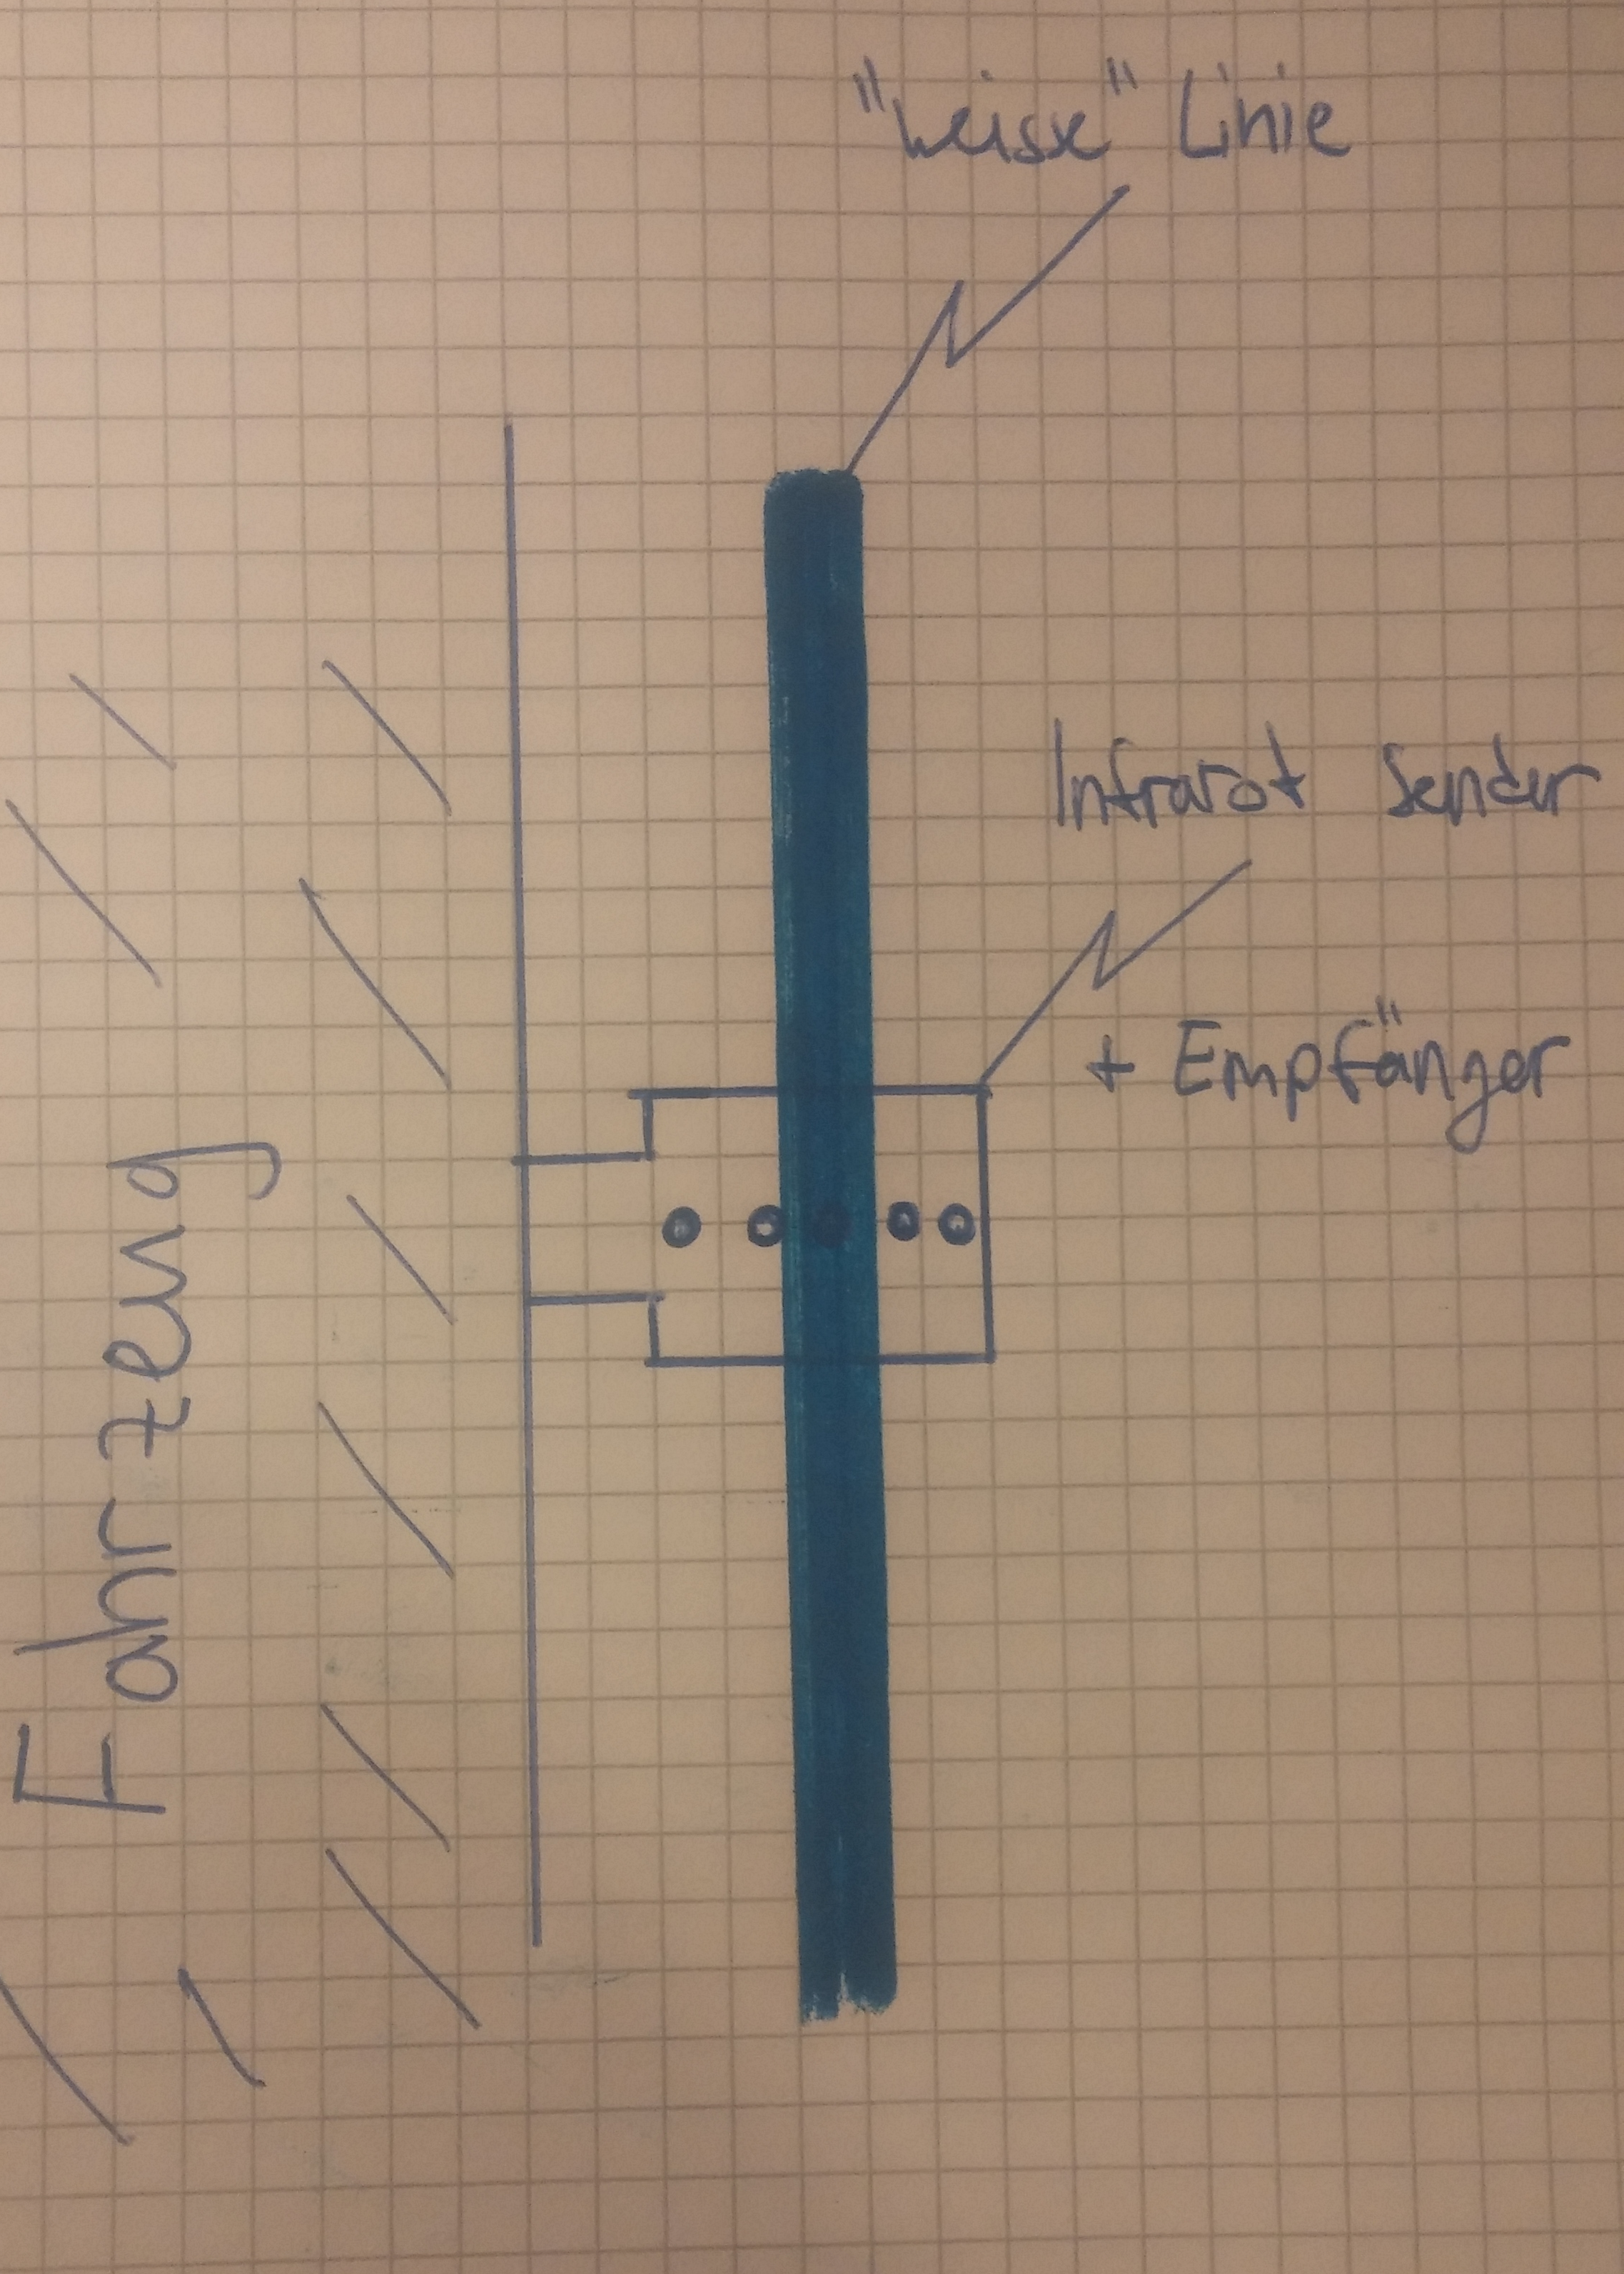
\includegraphics[width=\textwidth]{fig/Linienerkennung_1.png}
		\caption{1.Situation: Sensoren über der Linie}
	\end{subfigure}
	\hfill
	\begin{subfigure}[b]{0.36\textwidth}
		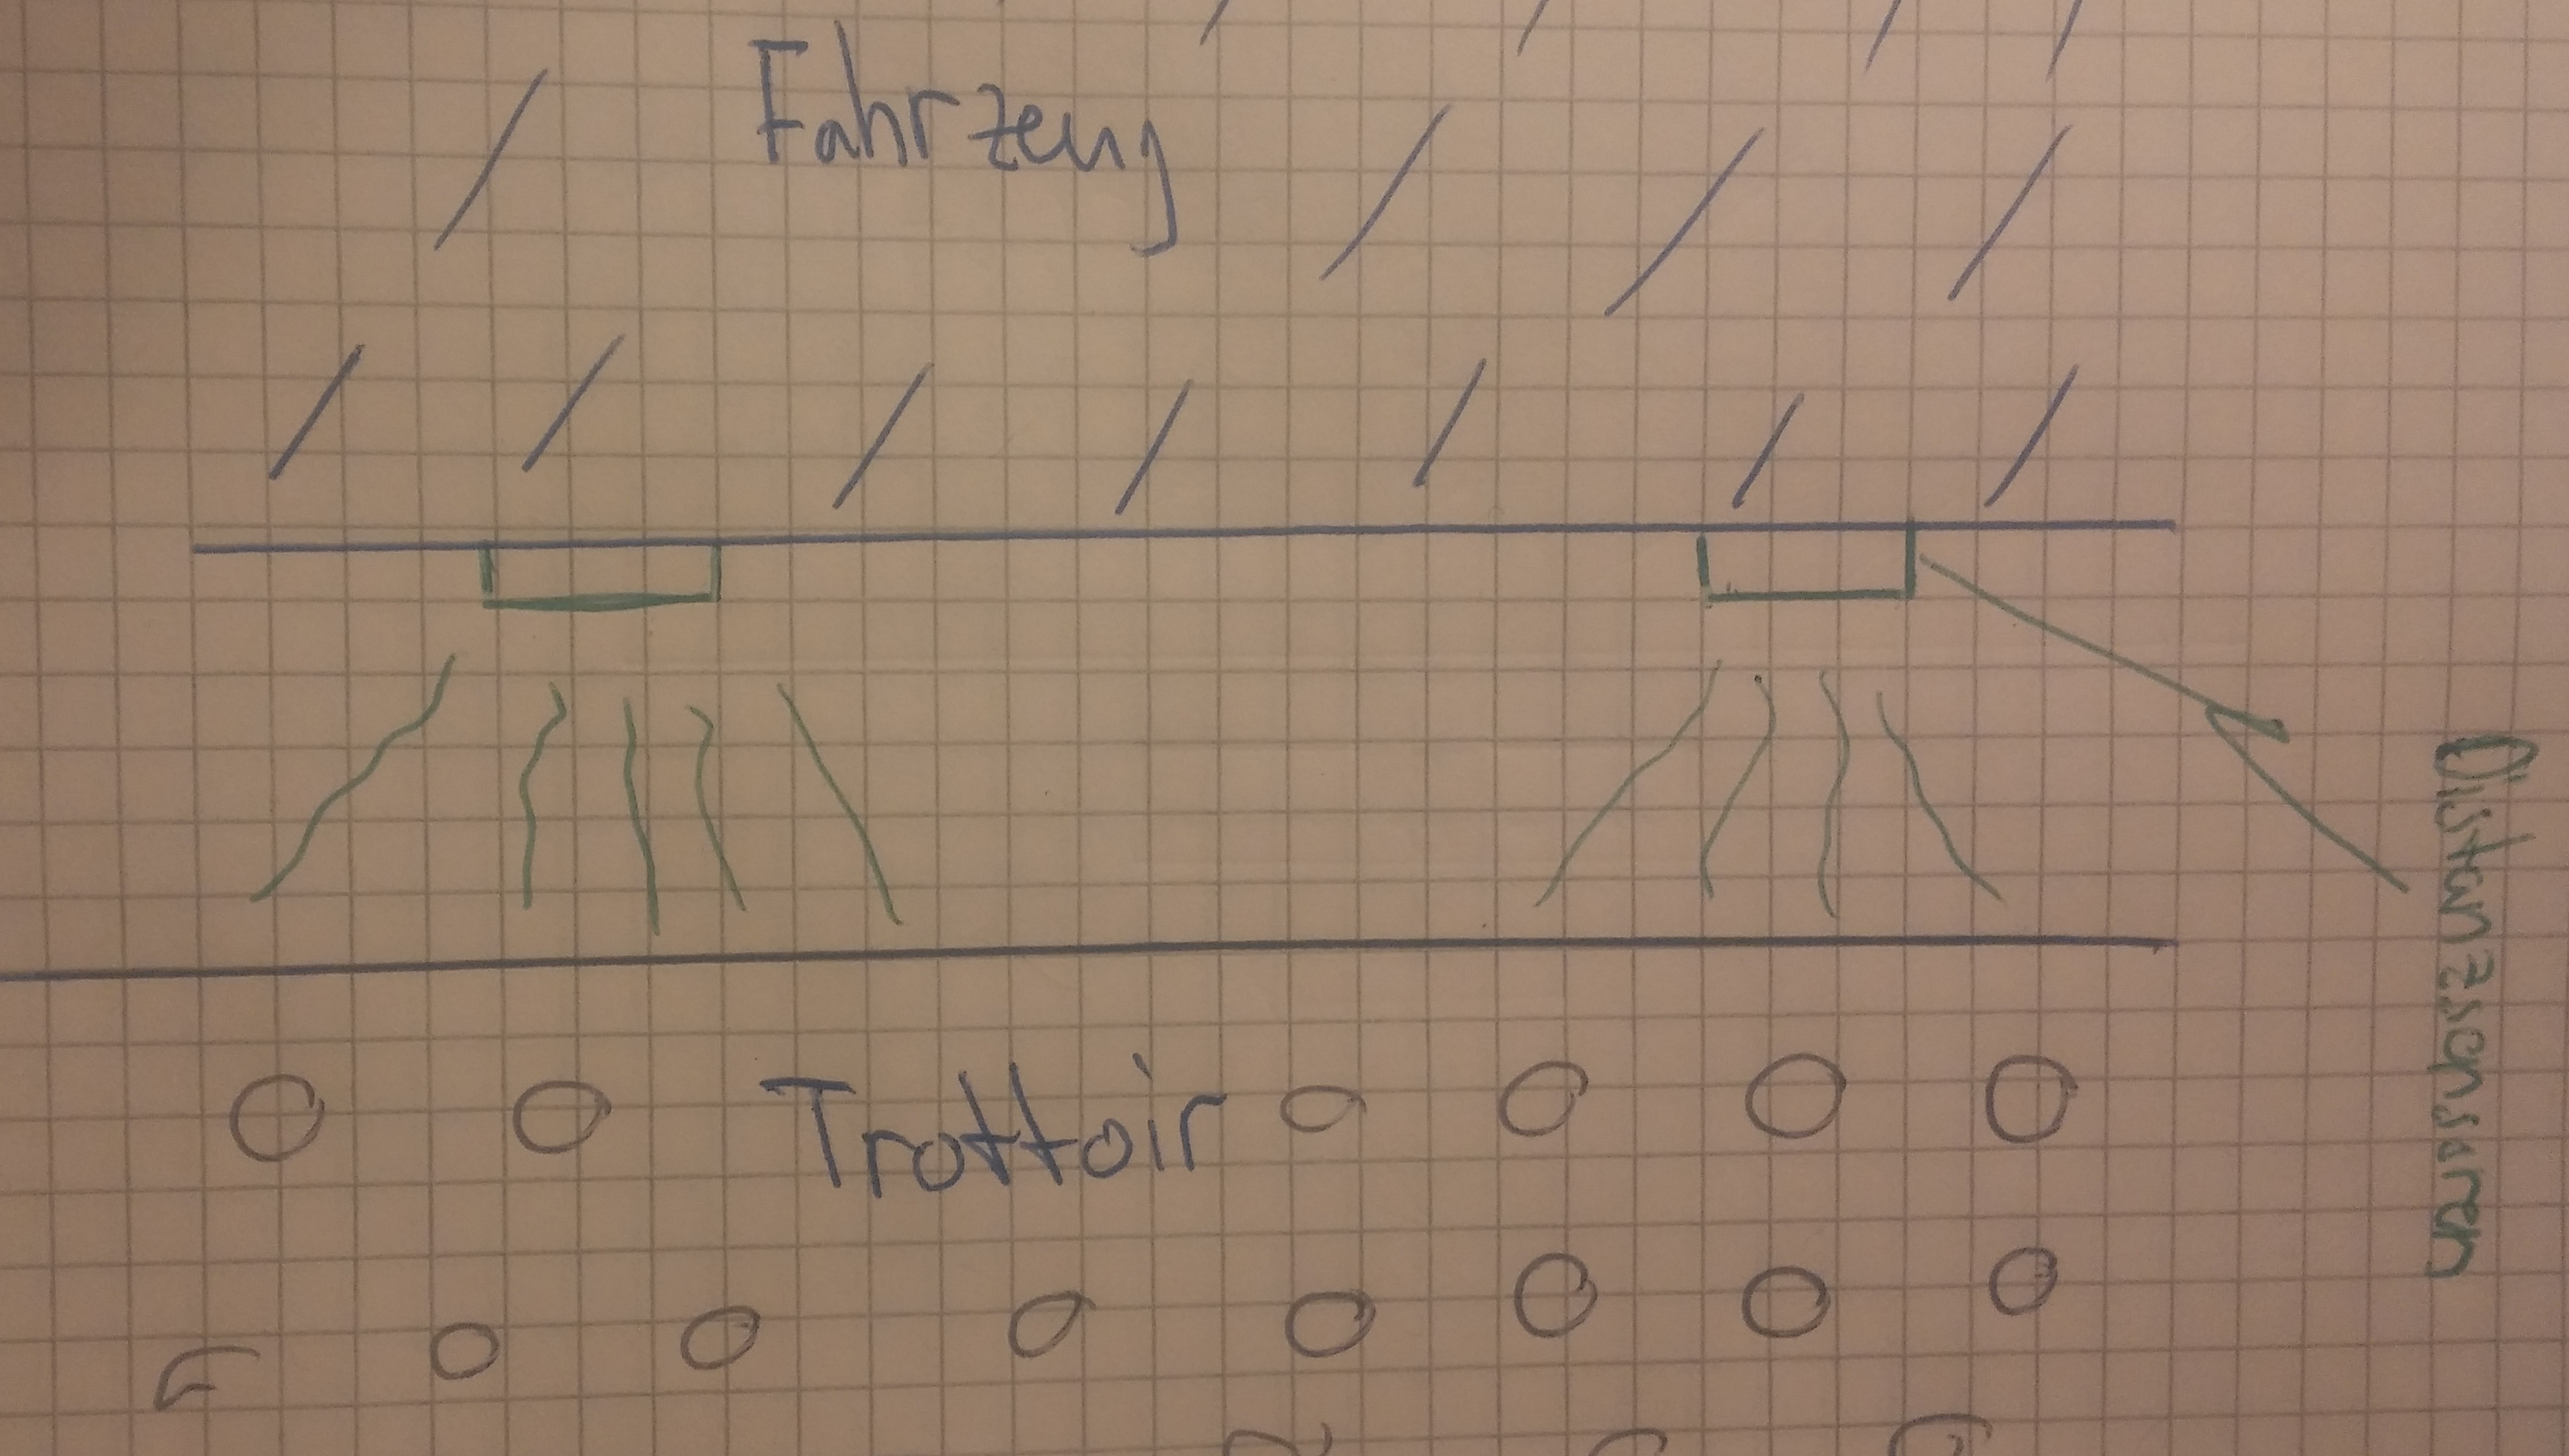
\includegraphics[width=\textwidth]{fig/Trottoirerkennung_1.png}
		\caption{2. Situation: Sensoren für die Abstandserkennung}
\end{subfigure}
	\caption{Mögliche Spurerkennung mit Distanzsensoren}\label{fig:animals}
\end{figure}



\begin{table}[h]
\begin{tabular}{p{0.5\textwidth} | p{0.5\textwidth}}


 \textbf{Vorteile} & \textbf{Nachteile} \\ \hline
	 
\begin{itemize}
\item Gut zu testen (Funktionsmuster)
\item Gute Präzision wird erwartet
\end{itemize}

 
 &
 
\begin{itemize}
\item Braucht externe Hardware und Verkabelung
\item Funktionsmuster zwingend notwendig
\end{itemize}

\end{tabular}
\end{table}

\begin{table}[h]
\begin{tabular}{p{0.5\textwidth}p{0.5\textwidth}}

 \textbf{Risiken} & \\ \hline
	 
\begin{itemize}
\item Die Linie lässt sich nicht Erkennen (ohne Konflikte mit der Anforderungsliste)
\item Das Trottoir ist zu wenig hoch damit es sich erkennen lässt
\end{itemize}
&
\begin{itemize}
\item Die Steuerung aufgrund der Linienerkennung ist nicht praktikabel
\end{itemize}

 
\end{tabular}
\end{table}

\pagebreak


%##############
\subsection{Bilderkennung}
Grafik

\begin{table}[h]
\begin{tabular}{p{0.5\textwidth} | p{0.5\textwidth}}


 \textbf{Vorteile} & \textbf{Nachteile} \\ \hline
	 
\begin{itemize}
\item Vorteil 1
\item Vorteil 2
\item Vorteil 3
\item ...
\end{itemize}

 
 &
 
\begin{itemize}
\item Nachteil 1
\item Nachteil 2
\item Nachteil 3
\item ...
\end{itemize}

\end{tabular}
\end{table}

\begin{table}[h]
\begin{tabular}{p{0.5\textwidth}p{0.5\textwidth}}


 \textbf{Risiken} & \\ \hline
	 
\begin{itemize}
\item Risiko 1
\item Risiko 2
\end{itemize}
&
\begin{itemize}
\item Risiko 3
\item ...
\end{itemize}

 
\end{tabular}
\end{table}

\pagebreak

% !TEX root = morphkasten.tex

\section{Containererkennung (grob)}


%##############
\subsection{Sensor}

\begin{figure} [hbp]
	\centering
	\includegraphics[width=0.5\textwidth]{fig/Containererkennung_2.png}
	\caption{Beispielhafte Containererkennung mit Sensoren}
\end{figure}

\begin{table}[h]
\begin{tabular}{p{0.5\textwidth} | p{0.5\textwidth}}


 \textbf{Vorteile} & \textbf{Nachteile} \\ \hline
	 
\begin{itemize}
\item Farberkennung möglich
\item Präzise Erkennung des Containers (wahrscheinlich)
\item Mehrfachverwendung mit anderen Anwendungen denkbar
\item Kostengünstig
\end{itemize}

 
 &
 
\begin{itemize}
\item Unbekannte Präzision
\item Je nach Sensor Störanfälligkeit
\item Zusatzhardware und Verkabelung nötig
\item 
\end{itemize}

\end{tabular}
\end{table}

\begin{table}[h]
\begin{tabular}{p{0.5\textwidth}p{0.5\textwidth}}


 \textbf{Risiken} & \\ \hline
	 
\begin{itemize}
\item Die Sensoren sind zu ungenau
\item Die Sensoren werden zu fest gestört
\end{itemize}
&
\begin{itemize}
\item Die Farbe kann auf Distanz nicht erkannt werden
\item Die Sensoren können zwischen Container und Sonstigem nicht unterscheiden
\end{itemize}

 
\end{tabular}
\end{table}

\pagebreak


%##############
\subsection{Bilderkennung}
\begin{figure}[h!]%Position festigen
\centering
\includegraphics[width=0.7\textwidth]{fig/containererkennung_grob_bilderkennung.png}
\caption{Bilderkennung Container}
\label{fig:Bilderkennung Container}
\end{figure}

\begin{table}[h]
\begin{tabular}{p{0.5\textwidth} | p{0.5\textwidth}}


\textbf{Vorteile} & \textbf{Nachteile} \\ \hline
	 
\begin{itemize}
\item bei grösserer Distanz zu Container schon erkennbar
\item Containererkennung durch Form- und/oder Farberkennung
\end{itemize}

 
 &
 
\begin{itemize}
\item Algorithmus nötig
\item rechenintensiv
\end{itemize}

\end{tabular}
\end{table}

\begin{table}[h]
\begin{tabular}{p{0.5\textwidth}p{0.5\textwidth}}

\textbf{Risiken} & \\ \hline
	 
\begin{itemize}
\item bei verschiedene Lichtverhätlnissen variieren die Farben
\item Container kann zum Teil von anderen Gegeständen verdeckt sein
\end{itemize}

 
\end{tabular}
\end{table}

\pagebreak

% !TEX root = morphkasten.tex

\section{Containererkennung (detailliert)}
Die Containererkennung muss auch ausgelegt sein für die Erkennung des Entladebehälters!

%##############
\subsection{Distanzsensor}
Die detaillierte Containererkennung mit Sensoren unterscheidet sich nur geringfügig von der groben Variante. Der Hauptunterschied besteht darin, dass bei der detaillierten Variante nur noch die Positionierung des Fahrzeugs vorzunehmen ist. Die Auswertung der Form und der Farbe wird Vorgängig von der Kamera erledigt und an das Mikrocontrollerboard weitergeleitet.
\begin{figure} [hbp]
	\centering
	\includegraphics[width=0.5\textwidth]{fig/Containererkennung_2.png}
	\caption{Beispielhafte Containererkennung mit Distanzsensoren (ohne Farbsensor)}
\end{figure}

\begin{table}[h]
\begin{tabular}{p{0.5\textwidth} | p{0.5\textwidth}}


 \textbf{Vorteile} & \textbf{Nachteile} \\ \hline
	 
\begin{itemize}
\item Präzise Erkennung des Containers (wahrscheinlich)
\item Mehrfachverwendung mit anderen Anwendungen denkbar
\item Kostengünstig (kein Farbsensor)
\end{itemize}

 
 &
 
\begin{itemize}
\item Unbekannte Präzision
\item Je nach Sensor Störanfälligkeit
\item Zusatzhardware und Verkabelung nötig
\end{itemize}

\end{tabular}
\end{table}

\begin{table}[h]
\begin{tabular}{p{0.5\textwidth}p{0.5\textwidth}}


 \textbf{Risiken} & \\ \hline
	 
\begin{itemize}
\item Die Sensoren sind zu ungenau
\item Die Sensoren werden gestört

\end{itemize}
&
\begin{itemize}
\item Die Kommunikation der groben und detaillierten Erkennung ist zu langsam
\end{itemize}

 
\end{tabular}
\end{table}

\pagebreak


%##############
\subsection{Bilderkennung}
\begin{figure}[h!]%Position festigen
\centering
\includegraphics[width=0.7\textwidth]{fig/containererkennung_detailliert_bilderkennung.png}
\caption{Bilderkennung Container}
\label{fig:Bilderkennung Container}
\end{figure}
\begin{table}[h]
\begin{tabular}{p{0.5\textwidth} | p{0.5\textwidth}}


 \textbf{Vorteile} & \textbf{Nachteile} \\ \hline
	 
\begin{itemize}
\item Keine Sensoren zur Seite benötigt
\end{itemize}

 
 &
 
\begin{itemize}
\item Berechnung des Abstands muss auf wenige Milimeter stimmen
\item Keine Korrektur mehr möglich, wenn der Container aus dem Kamerbereich verschwindet
\end{itemize}

\end{tabular}
\end{table}

\begin{table}[h]
\begin{tabular}{p{0.5\textwidth}p{0.5\textwidth}}


 \textbf{Risiken} & \\ \hline
	 
\begin{itemize}
\item Ungenauigkeit bei der Distanzabschätzung
\item Container kann zum Teil von anderen Gegeständen verdeckt sein
\end{itemize}

 
\end{tabular}
\end{table}

\pagebreak


% !TEX root = morphkasten.tex

\section{Rechtsvortritt}


%##############
\subsection{Sensor}

Grafik

\begin{table}[h]
\begin{tabular}{p{0.5\textwidth} | p{0.5\textwidth}}


 \textbf{Vorteile} & \textbf{Nachteile} \\ \hline
	 
\begin{itemize}
\item Vorteil 1
\item Vorteil 2
\item Vorteil 3
\item ...
\end{itemize}

 
 &
 
\begin{itemize}
\item Nachteil 1
\item Nachteil 2
\item Nachteil 3
\item ...
\end{itemize}

\end{tabular}
\end{table}

\begin{table}[h]
\begin{tabular}{p{0.5\textwidth}p{0.5\textwidth}}


 \textbf{Risiken} & \\ \hline
	 
\begin{itemize}
\item Risiko 1
\item Risiko 2
\end{itemize}
&
\begin{itemize}
\item Risiko 3
\item ...
\end{itemize}

 
\end{tabular}
\end{table}

\pagebreak


%##############
\subsection{Bilderkennung}

\begin{figure}[h!]%Position festigen
\centering
\includegraphics[width=0.7\textwidth]{fig/rechtsvortritt_bilderkennung.png}
\caption{Bilderkennung Rechtsvortritt}
\label{fig:Bilderkennung Rechtsvortritt}
\end{figure}

\begin{table}[h]
\begin{tabular}{p{0.5\textwidth} | p{0.5\textwidth}}


 \textbf{Vorteile} & \textbf{Nachteile} \\ \hline
	 
\begin{itemize}
\item Stoppen durch Vorausplnung möglich
\item Unterschiede berechnen, wie sich das andere Fahrzeug bewegt
\end{itemize}

 
 &
 
\begin{itemize}
\item Genaue Definition, was ein Fahzeug an der Kreuzung beim Rechtsvortritt ist
\item rechenintensiv
\end{itemize}

\end{tabular}
\end{table}

\begin{table}[h]
\begin{tabular}{p{0.5\textwidth}p{0.5\textwidth}}


\textbf{Risiken} & \\ \hline
	 
\begin{itemize}
\item Fahrzeug wird auch an anderen Stellen erkennt
\item andere Gegenstände könnten als Fahrzeug interpretiert werden

\end{itemize}

 
\end{tabular}
\end{table}

\pagebreak

% !TEX root = morphkasten.tex

\section{Programmiersprache}


%##############
\subsection{Java}

\begin{figure}[h!]%Position festigen
\centering
\includegraphics[width=0.5\textwidth]{fig/java.jpeg}
\caption{Java (Quelle: http://www.t3n.de)}
\label{fig:Java}
\end{figure}

\begin{table}[h]
\begin{tabular}{p{0.5\textwidth} | p{0.5\textwidth}}


 \textbf{Vorteile} & \textbf{Nachteile} \\ \hline
	 
\begin{itemize}
\item Objektorientiert
\item Unterstützt Multithreading
\item Plattformunabhängig
\end{itemize}

 
 &
 
\begin{itemize}
\item Langsamer als C++
\end{itemize}

\end{tabular}
\end{table}

\begin{table}[h]
\begin{tabular}{p{0.5\textwidth}p{0.5\textwidth}}


 \textbf{Risiken} & \\ \hline
	 
\begin{itemize}
\item Bilderkennung könnte zu langsam sein
\end{itemize}

 
\end{tabular}
\end{table}

\pagebreak


%##############
\subsection{C++}
\begin{figure}[h!]%Position festigen
\centering
\includegraphics[width=0.5\textwidth]{fig/cplusplus.png}
\caption{C++ (Quelle: http://www.unixstickers.com)}
\label{fig:C++}
\end{figure}
\begin{table}[h]
\begin{tabular}{p{0.5\textwidth} | p{0.5\textwidth}}


 \textbf{Vorteile} & \textbf{Nachteile} \\ \hline
	 
\begin{itemize}
\item Objektorientiert
\item Schneller als Java
\item In den meisten Tutorials von OpenCV wird mit C++ programmiert
\item Unterstützt Multithreading
\end{itemize}

 
 &
 
\begin{itemize}
\item Komplexer als Java
\end{itemize}

\end{tabular}
\end{table}

\begin{table}[h]
\begin{tabular}{p{0.5\textwidth}p{0.5\textwidth}}


 \textbf{Risiken} & \\ \hline
	 
\begin{itemize}
\item Komplexität
\end{itemize}

 
\end{tabular}
\end{table}

\pagebreak

% !TEX root = morphkasten.tex

\section{Bilderkennungs-Bibliothek}


%##############
\subsection{OpenCV}

\begin{figure}[h!]%Position festigen
\centering
\includegraphics[width=0.3\textwidth]{fig/opencv.png}
\caption{OpenCV (Quelle: https://en.wikipedia.org/wiki/OpenCV)}
\label{fig:OpenCV}
\end{figure}

\begin{table}[h]
\begin{tabular}{p{0.5\textwidth} | p{0.5\textwidth}}



 \textbf{Vorteile} & \textbf{Nachteile} \\ \hline
	 
\begin{itemize}
\item Grosse Community
\item Läuft auf Linux
\item Kostenlos
\item Kompatibel mit Java und C++
\end{itemize}

 
 &
 
\begin{itemize}
\item Enthält auch viele Funktionen, welche nicht benötigt werden (komplex)
\end{itemize}

\end{tabular}
\end{table}

\begin{table}[h]
\begin{tabular}{p{0.5\textwidth}p{0.5\textwidth}}


 \textbf{Risiken} & \\ \hline
	 
\begin{itemize}
\item Ressourcenknappheit
\end{itemize}

 
\end{tabular}
\end{table}

\pagebreak


%##############
\subsection{SimpleCV}
\begin{figure}[h!]%Position festigen
\centering
\includegraphics[width=0.5\textwidth]{fig/simplecv.png}
\caption{SimpleCV (Quelle: http://google-opensource.blogspot.ch/2012\_08\_01\_archive.html)}
\label{fig:SimpleCV}
\end{figure}

\begin{table}[h]
\begin{tabular}{p{0.5\textwidth} | p{0.5\textwidth}}


 \textbf{Vorteile} & \textbf{Nachteile} \\ \hline
	 
\begin{itemize}
\item Läuft auf Linux
\item Freie Software
\item Kompatibel mit Java und C++
\end{itemize}

 &
 
\begin{itemize}
\item Community kleiner als bei OpenCV
\end{itemize}

\end{tabular}
\end{table}

\begin{table}[h]
\begin{tabular}{p{0.5\textwidth}p{0.5\textwidth}}


\textbf{Risiken} & \\ \hline
	 
\begin{itemize}
\item Zu Problemen wird keine Lösung gefunden
\item Ressourcenknappheit
\end{itemize}
 
\end{tabular}
\end{table}

\pagebreak

\end{document}
% !TEX root = Technologierecherche.tex
\section{Recherchequellen}
\begin{tabular}{|p{3cm}|p{3.5cm}|p{5cm}|p{2cm}|}\hline
	
	\textbf{Themengebiet}	& 	\textbf{Beschreibung} & \textbf{Quelle} & \textbf{Bewertung (1-5)} \\\hline
	
	
	\textbf{Bilderkennung}	&	OpenCV Beschreibung	&	\url{http://docs.opencv.org/master/d1/dfb/intro.html#gsc.tab=0}	&	3 \\\hline
				 			&	Vergleich von OpenCV und SimpleCV	&	\url{http://simplecv.tumblr.com/post/19307835766/opencv-vs-matlab-vs-simplecv}	&	4 \\\hline
				 			&	SimpleCV Beschreibung	&	\url{http://simplecv.org/}	&	3 \\\hline
				 			&	Linienerkennung mit Open CV	&	\url{https://www.youtube.com/watch?v=aGGehlgiZoQ}	&	3	\\\hline
				 			
\textbf{Boardcomputer}	& 	Raspberry Pi & \url{https://www.pi-shop.ch/raspberry-pi-model-b} & 4 \\\hline
						& 	Raspberry Pi 2 & \url{https://www.pi-shop.ch/raspberry-pi-2-model-b} & 4 \\\hline
						& 	Banana Pi & \url{https://www.pi-shop.ch/banana-pi} & 4 \\\hline	
						
\textbf{Antrieb}	& 	Elektromotor & \url{http://www.modellbau-friedel.com} & 3 \\\hline
					& 	Verbrennungsmotor & \url{http://www.modellbau-friedel.com} & 3 \\\hline
					& 	Dampfmaschine & \url{www.modell-dampfmaschinen.de} & 3 \\\hline
					
\textbf{Lenkung} &  Beschreibung Knicklenkung und Bild & \url{http://www.portmanns.ch/Repetition/Fahrwerk/Lenkungsarten.pdf} & 3 \\\hline

& Beschreibung und Bild Achsschenkellenkung & \url{http://www.urlaub-und-hobby.de/metallbaukasten/so09dt.html} & 4 \\\hline 

& Lenktrapez & \url{http://portmanns.ch/Repetition/Fahrwerk/Achssch.pdf} & 2 \\\hline 

\textbf{Stromversorgung}	&	Vergleich von Akkutypen	&	\url{http://www.akku-abc.de/akku-vergleich.php}	&	3 \\\hline
				 			&	Grundlagenbeschreibung Akkutypen 	&	\url{http://rn-wissen.de/wiki/index.php/Akku-Grundlagen}	&	4 \\\hline
				 			&	Vergleich von Batterien und Akkus	&	\url{http://www.conrad.de/ce/de/content/ti_AkkusBatterien/Nickel-Zink-Akkus-die-neue-Alternative-zu-den-herkoemmlichen-Batterien}	&	3 \\\hline
				 			&	Vergleich von Batterien und Akkus	&	\url{http://www.computerbild.de/artikel/cb-Tests-PC-Hardware-Teure-Marken-gegen-Billig-Batterien-Mignon-AA-Micro-AAA-4640760.html } & 2	\\\hline
				 			
				 			
\textbf{Liniensensoren}	&	Beispiel eigene Liniensensoren mit Tipps	&	\url{http://www.cs.hs-rm.de/~linn/vpdv0708/asuro1/das_projekt_linienverfolgung.html}	&	3 \\\hline
\end{tabular}
\newpage
\begin{tabular}{|p{3cm}|p{3.5cm}|p{5cm}|p{2cm}|}\hline
				 			&	Opensource Beispiel Liniesensor	&	\url{https://www.tinkerforge.com/de/shop/bricklets/line-bricklet.html}	&	4 \\\hline
 				 			&	Opensource Beispiel Infrarot Linienfolger Arduino	&	\url{http://www.instructables.com/id/Arduino-Line-Following-Robot-for-Beginners/}	&	4 \\\hline
 				 			&	Opensource Beispiel Infrarot Linienfolger Selfmade + Regelung	&	\url{http://www.societyofrobots.com/member_tutorials/book/export/html/350}	&	2 \\\hline
 \textbf{Distanzsensoren}	&	Arduino Ulteraschallsensor Überblick &	\url{https://www.youtube.com/watch?v=U75vH-VfaPQ}	&	3 \\\hline	
 							&	Allgemeiner Sensor Überblick &	\url{http://www.robotc.de/ev3-sensoren/}	&	5 \\\hline	
 							&	IR Sensor (von Tinkerforge) &	\url{https://www.tinkerforge.com/de/shop/accessories/sensors/infrared-sensor-gp2y0a41sk0f.html}	&	1 \\\hline	
 							&	IR Sensor (von Tinkerforge, kurze Distanz) &	\url{http://www.tinkerforge.com/de/doc/Hardware/Bricklets/Line.html}	&	1 \\\hline	
 							
 							


\textbf{Farbsensor}	&	Farbsensormodul	&	\url{http://www.amazon.de/RGB-Farbsensor-mit-Filter-Arduino/dp/B00CYOFN2K}	&	3 \\\hline			 		
\textbf{Mikrocontroller Module}	&	MC Modul mit Erweiterungen	&	\url{https://www.tinkerforge.com/de/}	&	4 \\\hline
					&	Freedomboard	&	\url{http://www.freescale.com/products/arm-processors/kinetis-cortex-m:KINETIS}	&	5 \\\hline
					&	Freedomboard Übersicht KL-Line	&	\url{http://cache.freescale.com/files/microcontrollers/doc/selector_guide/KINETISLMCUSELGD.pdf?fpsp=1&WT_TYPE=Selecto}	&	4 \\\hline
					
					
					%20Guides&WT_VENDOR=FREESCALE&WT_FILE_FORMAT=pdf&WT_ASSET=Documentation&fileExt=.pdf
					&	Arduino Board &	\url{https://www.arduino.cc/en/Main/Boards}	&	2 \\\hline					
					
\textbf{Greifer}	& 	Beschreibung diverser Greifer & \url{http://www.zwahlenag.ch/produkte/greifer-pneumatische-greifzangen.php} & 3 \\\hline	
\textbf{Beladen}	& 	Video zu diversen Belademechanismen die in der Praxis verwendet werden & \url{https://www.youtube.com/watch?v=LTUjiLxzDQs} & 4 \\\hline
\textbf{Entladen}	& 	Bild einer möglichen Variante & \url{http://www.asia.ru/de/ProductInfo/1423164.html} & 2 \\\hline	
\textbf{Kamerasysteme} & Technische Doku Raspberry Pi CAM & \url{https://www.raspberrypi.org/documentation/hardware/camera.md} & 4 \\ \hline
                    & Logitech- Produkteseite Kamera  & \url{http://support.logitech.com/de_ch/home} & 2 \\ \hline
                    & Raspberry Pi Infrarotkamera & \url{https://www.raspberrypi.org/blog/pi-noir-infrared-camera-now-available/} & 2\\ \hline                    
\textbf{Spurerkennung Kamera} & Beispielvideo Spurerkennung & \url{http://weelug.blogspot.ch/2011/08/spurerkennung.html} & 2\\ \hline
                              & Infoseite iOnRoad App & \url{https://play.google.com/store/apps/details?id=com.picitup.iOnRoad} & 3\\ \hline
\end{tabular}\\
%% !TEX root = Technologierecherche.tex
\section{Schluss}
\end{document}